\chapter{Thực nghiệm so sánh trên tập dữ liệu MNIST}\label{chap:thucnghiemmnist}

Thực nghiệm đầu tiên sẽ là trên tập dữ liệu MNIST\footnote{THE MNIST DATABASE of handwritten digits, đường dẫn: \href{http://yann.lecun.com/exdb/mnist/}{http://yann.lecun.com/exdb/mnist/}}, xem xem những hàm kích hoạt khác nhau sẽ hoạt động thế nào  trong bài toán phân loại chữ số viết tay từ 0 tới 9.
Tập dữ liệu gồm 60,000 ảnh huấn luyện và 10,000 ảnh kiểm tra.
Mỗi ảnh là một ảnh xám có kích thước $28 \times 28 \times 1$, có điểm ảnh có giá trị ban đầu cao nhất là 255 và thấp nhất là 0, sau được chuẩn hoá lại về khoảng giá trị $[0, 1]$ bằng cách chia giá trị tất cả các điểm ảnh cho 255.
Trong quá trình huấn luyện, không sử dụng bất cứ kỹ thuật làm giàu dữ liệu nào.
Một lưu ý là, tập ảnh dữ liệu kiểm tra sẽ được dùng để kiểm định trong quá trình huấn luyện, tức ta sẽ bỏ qua quá trình kiểm tra và ta có thể xem như giá trị kiểm định cuối cùng là giá trị kiểm tra nếu muốn.
\vspace{5pt}

Các thông số của mạng như chiều sâu của mạng, kiểu khởi tạo trọng số, kích thước batch, tốc độ học, và thuật toán tối ưu đều có một ảnh hưởng nhất định lên quá trình huấn luyện một mô hình mạng học sâu.
Một số ảnh hưởng được đưa ra thử nghiệm để đánh giá như là việc tăng độ sâu của một mạng nơ-ron, thay đổi cách khởi tạo trọng số, thêm nhiễu vào dữ liệu, sử dụng kiến trúc mạng tích chập.
Đối với việc tăng độ sâu của mạng, kỹ thuật của mạng dư thừa không được áp dụng do cách thức trên sinh ra để xử lý việc tăng độ sâu của mạng, phần nào giảm đi tính đúng đắn về hiệu quả của các hàm kích hoạt.

\section{Thực nghiệm thông qua mạng nơ-ron sâu}\label{sec:mnistdl}

Bao gồm 11 kiến trúc được đưa ra, mỗi kiến trúc có số lượng tầng ẩn lần lượt tăng từ 2 cho tới 12.
Mỗi ảnh đầu vào sẽ được làm phẳng thành một vector có số chiều 728 (chính là $28 \times 28 \times 1 = 728$) tương ứng với số đơn vị ở tầng đầu vào.
Tầng đầu ra sẽ là 10 đơn vị ẩn tương ứng với 10 lớp từ 0 tới 9.
Các tầng ẩn sẽ có số lượng đơn vị ẩn như sau:

\begin{itemize}
    \item 2 tầng ẩn: $512 \rightarrow 128$.
    \item 3 tầng ẩn: $512 \rightarrow 256 \rightarrow 128$.
    \item 4 tầng ẩn: $512 \rightarrow 256 \rightarrow 128 \rightarrow 64$.
    \item 5 tầng ẩn: $512 \rightarrow 256 \rightarrow 128 \rightarrow 64 \rightarrow 32$.
    \item 6 tầng ẩn: $512 \rightarrow 256 \rightarrow 128 \rightarrow 64 \rightarrow 32 \rightarrow 16$.
    \item 7 tầng ẩn: $512(\times 2) \rightarrow 256 \rightarrow 128 \rightarrow 64 \rightarrow 32 \rightarrow 16$.
    \item 8 tầng ẩn: $512(\times 2) \rightarrow 256(\times 2) \rightarrow 128 \rightarrow 64 \rightarrow 32 \rightarrow 16$.
    \item 9 tầng ẩn: $512(\times 2) \rightarrow 256(\times 2) \rightarrow 128(\times 2) \rightarrow 64 \rightarrow 32 \rightarrow 16$.
    \item 10 tầng ẩn: $512(\times 2) \rightarrow 256(\times 2) \rightarrow 128(\times 2) \rightarrow 64(\times 2) \rightarrow 32 \rightarrow 16$.
    \item 11 tầng ẩn: $512(\times 2) \rightarrow 256(\times 2) \rightarrow 128(\times 2) \rightarrow 64(\times 2) \rightarrow 32(\times 2) \rightarrow 16$.
    \item 12 tầng ẩn: $512(\times 2) \rightarrow 256(\times 2) \rightarrow 128(\times 2) \rightarrow 64(\times 2) \rightarrow 32(\times 2) \rightarrow 16(\times 2)$.
\end{itemize}

Sau mỗi tầng dày đặc, một dropout có tỷ lệ 50\% sẽ được áp dụng, riêng với tầng ẩn cuối cùng của mỗi kiến trúc, tỷ lệ dropout giảm xuống 25\%.
\vspace{5pt}

Khi huấn luyện các mô hình với những hàm kích hoạt khác nhau, để cho công bằng thì khi cài đặt đều sử dụng chung một hàm tối ưu, tốc độ học và cùng một kiểu khởi tạo trọng số.
Kỹ thuật dropout cũng sẽ giống nhau nếu không có lưu ý gì.

\subsection{Dữ liệu không nhiễu và khởi tạo trọng số theo chuẩn hoá Lecun}\label{subsec:mnistd}

Tất cả được khởi tạo trọng số theo chuẩn hoá Lecun, riêng đối với mô hình áp dụng hàm kích hoạt SELU sẽ sử dụng kỹ thuật alpha dropout với tỷ lệ bằng với tỷ lệ dropout của các hàm kích hoạt khác.
Biểu đồ giá trị chính xác và mất mát trên tập kiểm định qua mỗi epoch được cho ở các hình \ref{fig:mnistd1}, \ref{fig:mnistd2}, \ref{fig:mnistd3}, \ref{fig:mnistd4}.
Chi tiết về giá trị được cho ở bảng \ref{tab:mnistdacc} và bảng \ref{tab:mnistdloss}.
Ở phần bảng giá trị không có thống kê của Sigmoid, do hàm này có kết quả tệ khá rõ rệt (sẽ được nêu rõ ngay sau đầy).
\vspace{5pt}

Với mạng nơ-ron không quá sâu - 2 tầng ẩn (hình \ref{fig:mnistd1a}, \ref{fig:mnistd1b}), các hàm dễ dàng đạt được độ chính xác cao (tất cả đều trên 92\%) và giá trị mất mát thấp (tất cả đều dưới 0.40).
Hàm Sigmoid không được tích cực giống như các hàm còn lại khi thua thiệt hẳn về tốc độ hội tụ khi mãi gần 20 epoch mới đạt được mất mát dưới giá trị 1.
Tuy các hàm ngoài Sigmoid chưa thấy được sự khác biệt rõ rệt, nhưng có vẻ như SELU là người yếu thế nhất trong nhóm này khi giá trị mất mát tuy hội tụ khá sớm.
Chỉ sau 20 epoch (bảng \ref{tab:mnistdepoch}), 80\% giá trị mất mát đã bằng giá trị mất mát cuối cùng.
Nhưng kết quả mất mát cuối cùng không quá ấn tượng và gần bằng so với Sigmoid.
\vspace{5pt}

Ngay khi tăng lên 3 tầng ẩn (hình \ref{fig:mnistd1c}, \ref{fig:mnistd1d}), Sigmoid đã cho thấy sự lép vế rõ rệt.
Không chỉ thế, SELU cũng có vẻ sẽ chung số phận với Sigmoid khi số lượng tầng ẩn tiếp tục tăng.
Dù cho cuối cùng SELU vẫn đạt giá trị chính xác trên 92\% nhưng giá trị mất mát đã tiệm cận 0.50 (chính xác là 0.49).
\vspace{5pt}

Sigmoid chính thức bỏ cuộc khỏi cuộc đua khi tới số tầng ẩn là 5 (hình \ref{fig:mnistd2a}, \ref{fig:mnistd2b}), gần như mô hình với hàm này không thể học được.
SELU tuy vẫn còn có khả năng học, nhưng cho kết quả rất tệ như Sigmoid những mô hình ban đầu khi giá trị mất mát đạt tới 1.67.
Dù cho vẫn giữ được độ chính xác gần 90\%, nhưng khi tăng thêm số tầng ẩn thì có khả năng cao sẽ bị giảm đi thấp rất nhiều.
Ngoài ra, ta thấy rằng hàm ELU và Tanh có vẽ hội tụ nhanh hơn so với các hàm còn lại, và chính xác là như thế khi ELU chỉ cần đúng 3 epoch để 80\% mất mát hiện tại bằng mất ngưỡng.
Với Tanh thì con số này là 24 epoch.
Kế đến là Leaky và RELU ngay sau (cùng 27 epoch), Swish (38) và GELU (35) ở nhóm sau cùng.
Giá trị chính xác và mất mát của các hàm kích hoạt sau 50 epoch vẫn chưa có sự chênh lệch đáng kể.
\vspace{5pt}

Độ sâu được nâng lên 7 tầng ẩn (hình \ref{fig:mnistd2e}, \ref{fig:mnistd2f}), Leaky đã bỏ lại RELU chung với nhóm của GELU và Swish ở khoảng 15 epoch đầu tiên.
Mãi khi về cuối, RELU cũng như GELU và Swish mới bám được với nhóm dẫn đầu gồm có ELU, Tanh và Leaky.
Lúc này, vẫn chưa có sự chênh lệch quá đáng kể về giá trị chính xác cũng như mất mát.
Duy chỉ có Swish có vẻ đuối sức so với những hàm còn lại khi giá trị chính xác duy trì được $\approx$ 95\% giảm xuống 92.03\%.
SELU lúc này đã không còn có khả năng tiếp tục khi giá trị chính xác giảm thảm hại xuống 37.25\% và giá trị mất mát là 7.02.
So với lúc 5 tầng ẩn thì đã giá trị chính xác đã giảm đi 50\%, giá trị mất mát thì tăng lên 5.35.
\vspace{5pt}

Kết quả khi số tầng ẩn tăng lên là 9 (hình \ref{fig:mnistd3c}, \ref{fig:mnistd3d}) cho thấy chỉ có Leaky, Elu và Tanh là đủ sức để đi tiếp những mô hình sâu hơn khi vẫn giữ được giá trị chính xác trên 90\%.
Trong nhóm này, ELU có vẻ nổi trội hơn một chút so với hai hàm còn lại ở những epoch đầu.
Dẫu thế, những kết quả về cuối cho thấy ELU vẫn chưa thể tách nhóm khi giá trị chính xác vẫn chỉ đang xấp xỉ Leaky.
Nhóm còn lại gồm RELU, GELU và Swish thì chỉ có RELU và GELU tiếp tục khi Swish cũng cho thấy sự hụt hơi của mình (chính xác: 57.32\%, mất mát: 1.21).
Tuy nhiên ở ngay độ sâu kế tiếp - 10 tầng ẩn (hình \ref{fig:mnistd3e}, \ref{fig:mnistd3f}), GELU cũng như Swish đã không còn có khả năng học được nữa khi giá trị chính xác cũng như mất mát đã bão hoà ở mức 10.60\% và 2.30.
\vspace{5pt}

Ở mô hình cuối cùng - 12 tầng ẩn (hình \ref{fig:mnistd4c}, \ref{fig:mnistd4d}), Leaky lúc này cũng không còn bám được với nhóm đầu dù là những epoch cuối khi giá trị tụt xuống 62.84\% và mất mát 1.08.
Nhà vô địch ở mô hình này là ELU với chiến thắng khá thuyết phục khi ta thấy có cách biệt rõ rệt giữa ELU so với Tanh và cụ thể là giá trị chính xác 79.24\% > 76.97\%, giá trị mất mát 0.45 < 0.6.
Tốc độ hội tụ của ELU cũng nhanh hơn rõ rệt khi sau 16 epoch đã đạt được giá trị cần thiết so với Tanh cần tới 26 epoch.

\begin{table}[ht!]
\centering
\def\arraystretch{1.1}
\begin{tabular}{c|c|c|c|c|c|c|c|c|c|c|c|}
\cline{2-12}
& 2     & 3     & 4     & 5     & 6     & 7     & 8     & 9     & 10    & 11    & 12    \\ \hline
\multicolumn{1}{|c|}{$\tanh$} & 93.87 & 94.77 & 95.15 & 94.86 & 94.55 & 94.87 & 94.61 & 94.55 & 94.66 & 94.64 & 76.97 \\ \hline
\multicolumn{1}{|c|}{$\mathcal{R}$} & \textbf{96.87} & \textbf{97.13} & \textbf{97.39} & \textbf{97.32} & 96.66 & 96.16 & 95.33 & 79.99 & 79.18 & 42.32 & 37.99 \\ \hline
\multicolumn{1}{|c|}{$\mathcal{R}_L$} & 96.22 & 96.82 & 97.12 & 96.78 & \textbf{96.70} & \textbf{97.02} & \textbf{97.01} & \textbf{96.39} & \textbf{96.64} & 87.16 & 62.84 \\ \hline
\multicolumn{1}{|c|}{$\mathcal{E}$} & 94.79 & 95.76 & 95.99 & 95.92 & 95.43 & 95.84 & 95.92 & 95.92 & 95.67 & \textbf{95.45} & \textbf{79.24} \\ \hline
\multicolumn{1}{|c|}{$\mathcal{E}_S$} & 92.85 & 92.68 & 91.47 & 87.25 & 65.71 & 37.25 & 30.75 & 27.47 & 10.79 & 10.87 & 10.60 \\ \hline
\multicolumn{1}{|c|}{$\mathcal{G}$} & 96.03 & 96.28 & 96.29 & 96.38 & 95.05 & 94.69 & 92.58 & 80.23 & 10.60 & 10.60 & 10.60 \\ \hline
\multicolumn{1}{|c|}{$\mathcal{S}$} & 95.13 & 95.51 & 95.39 & 95.38 & 93.07 & 92.03 & 88.86 & 57.32 & 10.60 & 10.60 & 10.60 \\ \hline
\end{tabular}
\caption{Giá trị chính xác (\%) của các hàm kích hoạt (chuẩn hoá Lecun) tương ứng với các số tầng ẩn của mô hình trên tập dữ liệu MNIST.}
\label{tab:mnistdacc}
\end{table}

\begin{table}[ht!]
\centering
\def\arraystretch{1.3}
\begin{tabular}{c|c|c|c|c|c|c|c|c|c|c|c|}
\cline{2-12}
                        & 2    & 3    & 4    & 5    & 6    & 7    & 8    & 9    & 10   & 11   & 12   \\ \hline
\multicolumn{1}{|c|}{$\tanh$} & 0.21 & 0.19 & 0.17 & 0.19 & 0.22 & 0.21 & 0.23 & 0.24 & 0.26 & 0.27 & 0.60  \\ \hline
\multicolumn{1}{|c|}{$\mathcal{R}$} & \textbf{0.11} & \textbf{0.09} & \textbf{0.09} & \textbf{0.11} & 0.16 & 0.28 & 0.33 & 0.53 & 0.57 & 1.21 & 1.39 \\ \hline
\multicolumn{1}{|c|}{$\mathcal{R}_L$} & 0.13 & 0.11 & 0.10 & 0.12 & \textbf{0.13} & \textbf{0.13} & \textbf{0.13} & 0.17 & 0.19 & 0.37 & 1.08 \\ \hline
\multicolumn{1}{|c|}{$\mathcal{E}$} & 0.19 & 0.15 & 0.14 & 0.15 & 0.17 & 0.16 & 0.16 & \textbf{0.16} & \textbf{0.18} & \textbf{0.20} & \textbf{0.45} \\ \hline
\multicolumn{1}{|c|}{$\mathcal{E}_S$} & 0.38 & 0.49 & 0.81 & 1.67 & 2.79 & 7.02 & 7.55 & 4.86 & 2.30  & 2.30  & 2.30  \\ \hline
\multicolumn{1}{|c|}{$\mathcal{G}$} & 0.14 & 0.12 & 0.12 & 0.13 & 0.20 & 0.22 & 0.34 & 0.72 & 2.30  & 2.30  & 2.30  \\ \hline
\multicolumn{1}{|c|}{$\mathcal{S}$} & 0.17 & 0.16 & 0.15 & 0.16 & 0.29 & 0.36 & 0.46 & 1.21 & 2.30  & 2.30  & 2.30  \\ \hline
\end{tabular}
\caption{Giá trị mất mát của các hàm kích hoạt (chuẩn hoá Lecun) tương ứng với các mô hình trên tập dữ liệu MNIST.}
\label{tab:mnistdloss}
\end{table}

\begin{table}[ht!]
\centering
\def\arraystretch{1.3}
\begin{tabular}{c|c|c|c|c|c|c|c|c|c|c|c|c|}
\cline{2-13}
                        & 2  & 3  & 4  & 5  & 6  & 7  & 8  & 9  & 10 & 11 & 12 & $\mu$ \\ \hline
\multicolumn{1}{|c|}{$\tanh$} & \textbf{19} & \textbf{22} & 30 & \textbf{24} & \textbf{26} & \textbf{27} & \textbf{30} & \textbf{30} & \textbf{26} & \textbf{27} & 26 & \textbf{26}\\ \hline
\multicolumn{1}{|c|}{$\mathcal{R}$} & 33 & 34 & 31 & 27 & 38 & 36 & 34 & 31 & 33 & 23 & 27 & 32\\ \hline
\multicolumn{1}{|c|}{$\mathcal{R}_L$} & 32 & 31 & 32 & 27 & 33 & 31 & 31 & 34 & 39 & 46 & 27 & 33\\ \hline
\multicolumn{1}{|c|}{$\mathcal{E}$} & 26 & 33 & 32 & 28 & 28 & 30 & 32 & 31 & 30 & 26 & \textbf{16} & 28\\ \hline
\multicolumn{1}{|c|}{$\mathcal{E}_S$} & 20 & \textbf{22} & \textbf{16} & 3  & 1  & 1  & 1  & 1  & 1  & 1  & 1  & X\\ \hline
\multicolumn{1}{|c|}{$\mathcal{G}$} & 32 & 35 & 35 & 35 & 38 & 43 & 42 & 45 & 1  & 1  & 1  & X\\ \hline
\multicolumn{1}{|c|}{$\mathcal{S}$} & 33 & 32 & 37 & 38 & 40 & 39 & 43 & 43 & 1  & 1  & 1  & X\\ \hline
\end{tabular}
\caption{Số epoch cần thiết để 80\% giá trị mất mát (chuẩn hoá Lecun) bằng giá trị mất mát cuối cùng.}
\label{tab:mnistdepoch}
\end{table}

\begin{table}[ht!]
\centering
\def\arraystretch{1.5}
\begin{tabular}{c|c|c|c|c|c|c|c|}
\cline{2-8}
                             & $\tanh$      & $\mathcal{R}$      & $\mathcal{R}_L$      & $\mathcal{E}$      & $\mathcal{E}_S$      & $\mathcal{G}$      & $\mathcal{S}$      \\ \hline
\multicolumn{1}{|c|}{$\mu_{\text{chính xác}}$ (\%)}    & 93.05  & 83.31  & 92.77  & \textbf{94.18}  & 50.7   & 70.85  & 67.68  \\ \hline
\multicolumn{1}{|c|}{$\sigma^2_{\text{chính xác}} (\%)$}  & 0.0026 & 0.0456 & 0.0097 & \textbf{0.0022} & 0.1152 & 0.1380 & 0.1330 \\ \hline
\multicolumn{1}{|c|}{$\mu_{\text{mất mát}}$}   & 0.25   & 0.44   & 0.24   & \textbf{0.19}   & 2.95   & 0.81   & 0.9    \\ \hline
\multicolumn{1}{|c|}{$\sigma^2_{\text{mất mát}}$} & 0.0131 & 0.1907 & 0.0748 & \textbf{0.0069} & 5.5967 & 0.8616 & 0.8204 \\ \hline
\end{tabular}
\caption{Giá trị trung bình và phương sai của các hàm kích hoạt (chuẩn hoá Lecun) trong 11 mô hình thử nghiệm.}
\label{tab:mnistdmean}
\end{table}

Độ sâu của mạng tăng thì ảnh hưởng nhiều tới giá trị chính xác hơn là so với giá trị mất mát khi giá trị chính xác có những góc gãy bớt tù hơn so với giá trị mất mát (hình \ref{fig:mnistd4e}, \ref{fig:mnistd4f}).
Theo bảng \ref{tab:mnistdacc} và bảng \ref{tab:mnistdloss}, ở những mạng chưa quá sâu, RELU là hàm có kết quả tốt nhất.
Khi mạng sâu hơn một chút thì Leaky là hàm dẫn đầu, nhưng khi mạng trở nên phức tạp hơn với khoảng 9 tầng ẩn thì Leaky không còn đạt được phong độ tốt nữa mà thay vào đó là ELU.
Có 2 hàm rất bền bỉ từ những mạng đầu tiên là ELU và Tanh.
Trong đó, Tanh luôn tìm được điểm cực tiểu sớm nhất (bảng \ref{tab:mnistdepoch}) bất kể độ sâu của mạng.
Nhưng điều này cũng chưa cho thấy Tanh thực sự tốt hơn RELU hay Leaky, lí do có thể là vì Tanh chỉ đang tìm được hố cực tiẻu nông, trong khi RELU hay Leaky tìm thấy một hố cực tiểu sâu hơn để có giá trị tốt hơn.
Mãi khi mạng quá sâu, RELU và Leaky không thể tìm được hố cực tiểu tốt nữa, thì lúc đó hố cực tiểu của Tanh nghiễm nhiên trở thành một giá trị tốt hơn.
\vspace{5pt}

Theo như bảng \ref{tab:mnistdmean}, có 3 hàm đạt được giá trị chính xác trung bình $\mu_{\text{chính xác}}$ trong 11 mô hình trên 90\% lần lượt từ thấp tới cao là Leaky, Tanh và ELU.
Phương sai về chính xác $\sigma^2_{\text{chính xác}}$ và mất mát $\sigma^2_{\text{mất mát}}$ của Leaky cao hơn so với Tanh với ELU là do ở những tầng cuối thì thông số của Leaky thay đổi nhiều khi giá trị chính xác giảm đáng kể dù cho mất mát tăng không quá căng thẳng.
\vspace{5pt}

Hàm Sigmoid thực sự không phù hợp để huấn luyện cho những mạng học sâu đúng với nhưng suy tính lý thuyết, vì thế các thực nghiệm tiếp theo sẽ không có hàm Sigmoid.

\begin{figure}[ht!]
     \begin{center}
%
        \subfigure[Giá trị chính xác tập kiểm định (2)]{%
            \label{fig:mnistd1a}
            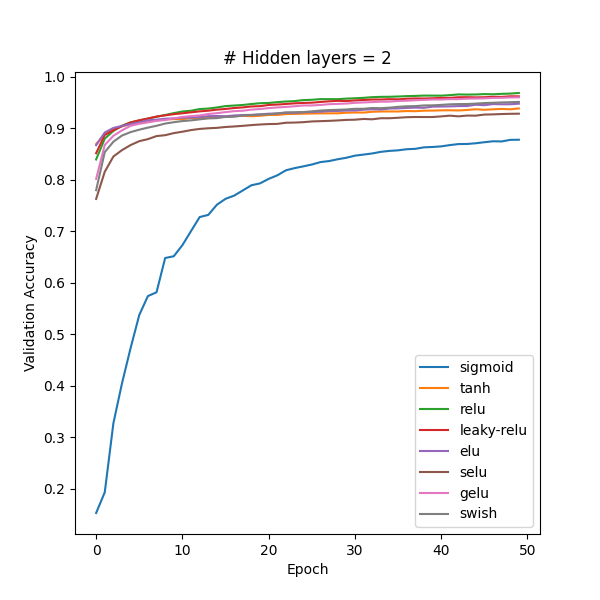
\includegraphics[width=0.4\textwidth]{images/2_hidden_layers_acc.png}
        }%
        \subfigure[Giá trị mất mát tập kiểm định (2)]{%
           \label{fig:mnistd1b}
           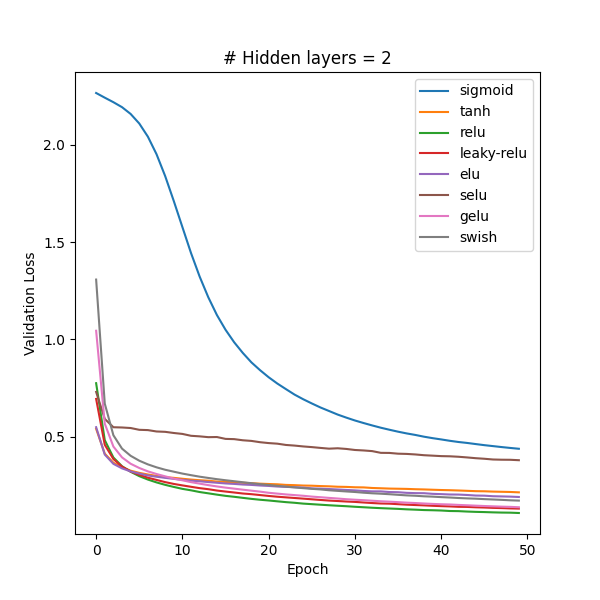
\includegraphics[width=0.4\textwidth]{images/2_hidden_layers_loss.png}
        }\\ %  ------- End of the first row ----------------------%
        \subfigure[Giá trị chính xác tập kiểm định (3)]{%
            \label{fig:mnistd1c}
            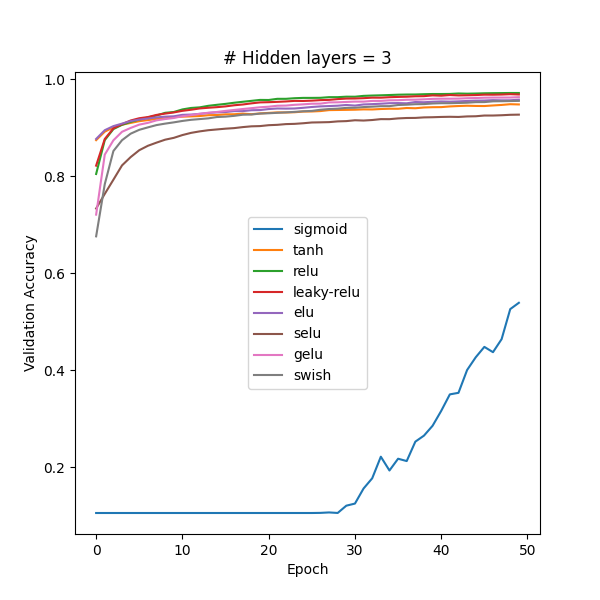
\includegraphics[width=0.4\textwidth]{images/3_hidden_layers_acc.png}
        }%
        \subfigure[Giá trị mất mát tập kiểm định (3)]{%
            \label{fig:mnistd1d}
            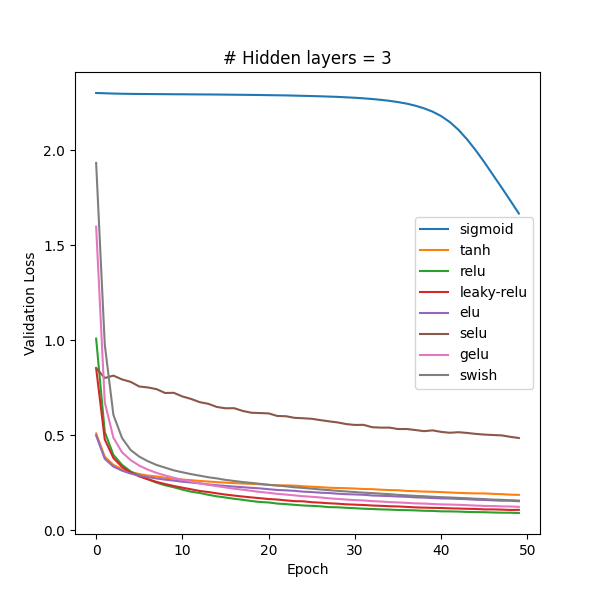
\includegraphics[width=0.4\textwidth]{images/3_hidden_layers_loss.png}
        }\\
        %----------------------%
        \subfigure[Giá trị chính xác tập kiểm định (4)]{%
            \label{fig:mnistd1e}
            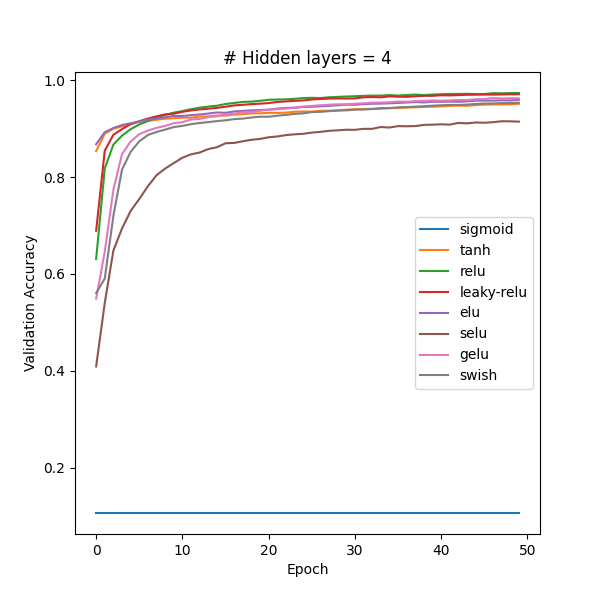
\includegraphics[width=0.4\textwidth]{images/4_hidden_layers_acc.png}
        }%
        \subfigure[Giá trị mất mát tập kiểm định (4)]{%
            \label{fig:mnistd1f}
            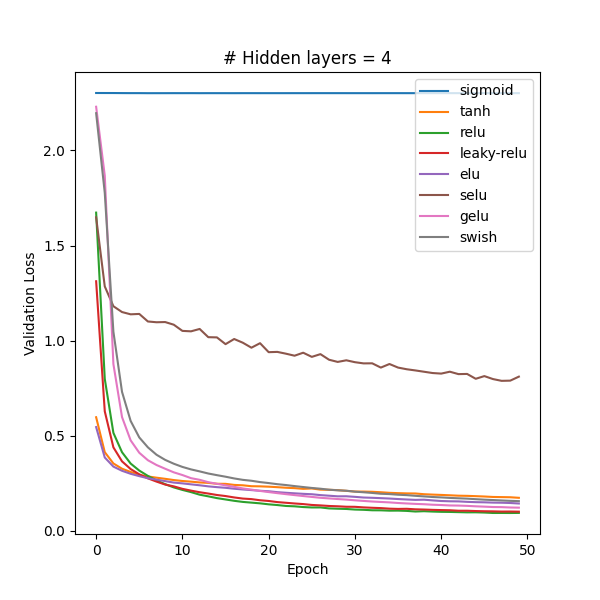
\includegraphics[width=0.4\textwidth]{images/4_hidden_layers_loss.png}
        }%
%
    \end{center}
    \caption{%
        Giá trị chính xác và mất mát (chuẩn hoá Lecun) trên tập kiểm định (số tầng ẩn: 2, 3, 4).
     }%
   \label{fig:mnistd1}
\end{figure}

\begin{figure}[ht!]
     \begin{center}
%
        \subfigure[Giá trị chính xác tập kiểm định (5)]{%
            \label{fig:mnistd2a}
            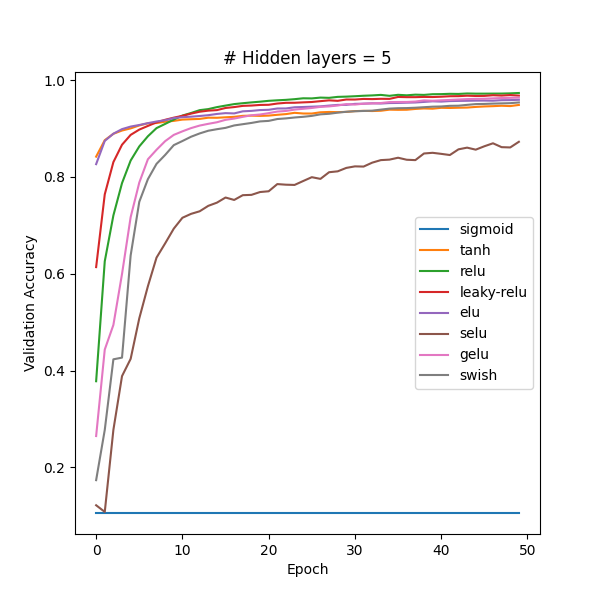
\includegraphics[width=0.4\textwidth]{images/5_hidden_layers_acc.png}
        }%
        \subfigure[Giá trị mất mát tập kiểm định (5)]{%
           \label{fig:mnistd2b}
           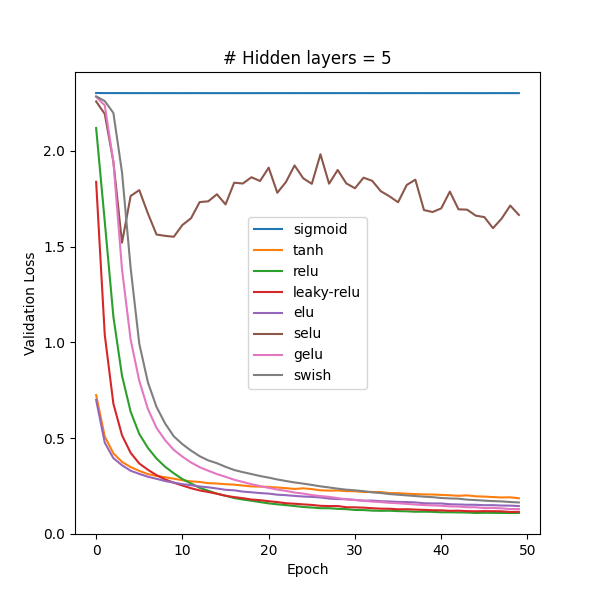
\includegraphics[width=0.4\textwidth]{images/5_hidden_layers_loss.png}
        }\\ %  ------- End of the first row ----------------------%
        \subfigure[Giá trị chính xác tập kiểm định (6)]{%
            \label{fig:mnistd2c}
            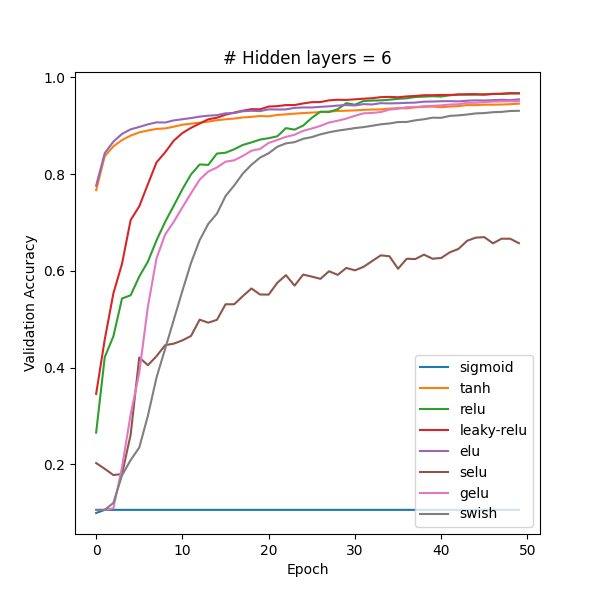
\includegraphics[width=0.4\textwidth]{images/6_hidden_layers_acc.png}
        }%
        \subfigure[Giá trị mất mát tập kiểm định (6)]{%
            \label{fig:mnistd2d}
            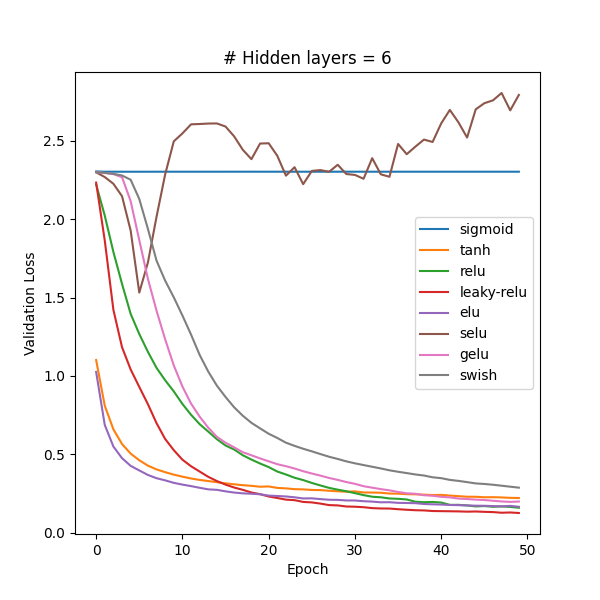
\includegraphics[width=0.4\textwidth]{images/6_hidden_layers_loss.png}
        }\\
        %----------------------%
        \subfigure[Giá trị chính xác tập kiểm định (7)]{%
            \label{fig:mnistd2e}
            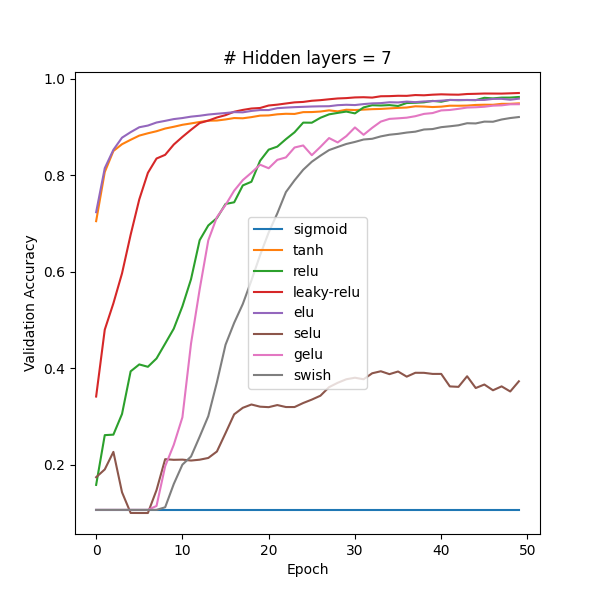
\includegraphics[width=0.4\textwidth]{images/7_hidden_layers_acc.png}
        }%
        \subfigure[Giá trị mất mát tập kiểm định (7)]{%
            \label{fig:mnistd2f}
            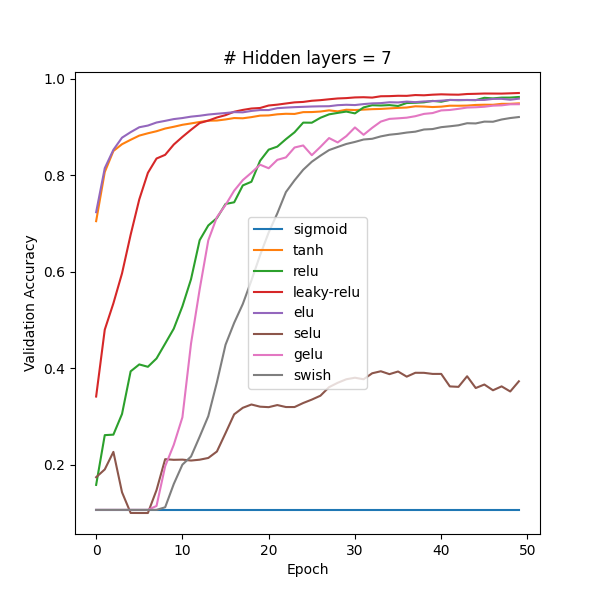
\includegraphics[width=0.4\textwidth]{images/7_hidden_layers_acc.png}
        }%
%
    \end{center}
    \caption{%
        Giá trị chính xác và mất mát (chuẩn hoá Lecun) trên tập kiểm định (số tầng ẩn: 5, 6, 7).
     }%
   \label{fig:mnistd2}
\end{figure}

\begin{figure}[ht!]
     \begin{center}
%
        \subfigure[Giá trị chính xác tập kiểm định (8)]{%
            \label{fig:mnistd3a}
            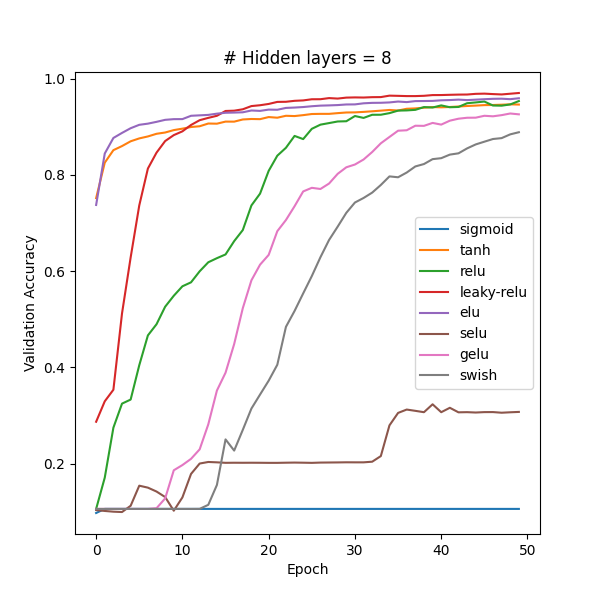
\includegraphics[width=0.4\textwidth]{images/8_hidden_layers_acc.png}
        }%
        \subfigure[Giá trị mất mát tập kiểm định (8)]{%
           \label{fig:mnistd3b}
           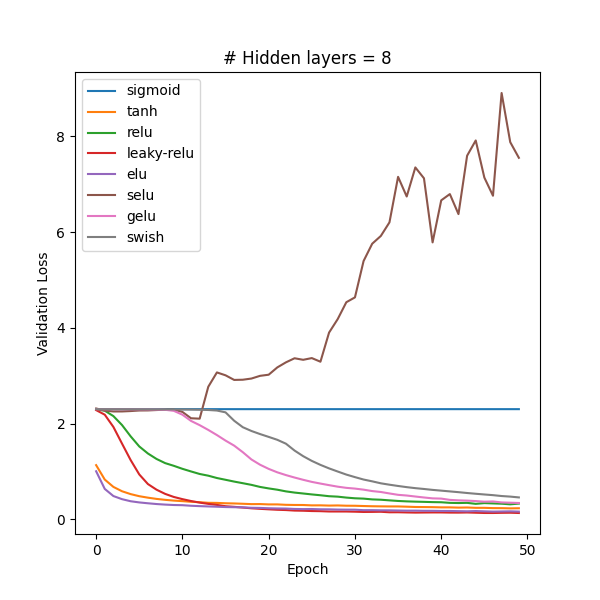
\includegraphics[width=0.4\textwidth]{images/8_hidden_layers_loss.png}
        }\\ %  ------- End of the first row ----------------------%
        \subfigure[Giá trị chính xác tập kiểm định (9)]{%
            \label{fig:mnistd3c}
            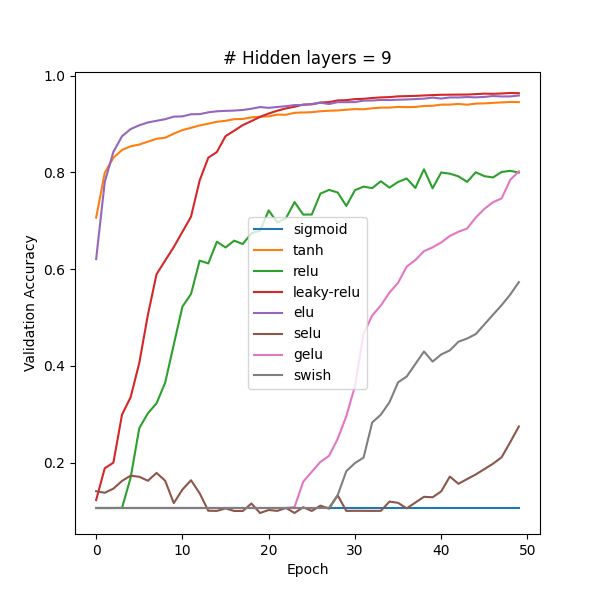
\includegraphics[width=0.4\textwidth]{images/9_hidden_layers_acc.png}
        }%
        \subfigure[Giá trị mất mát tập kiểm định (9)]{%
            \label{fig:mnistd3d}
            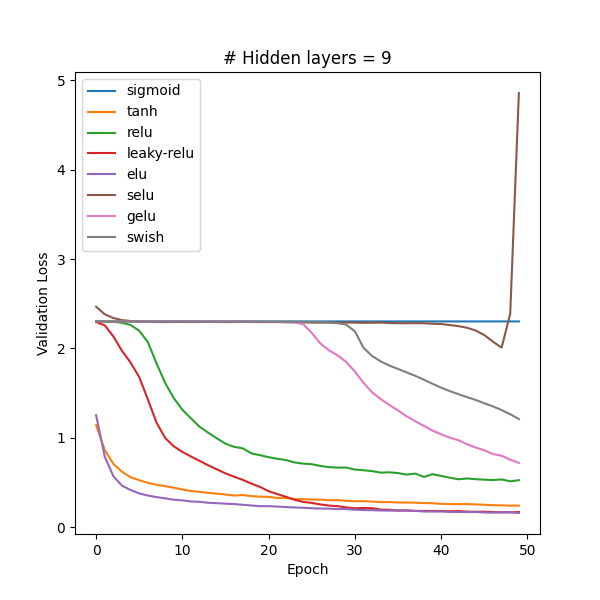
\includegraphics[width=0.4\textwidth]{images/9_hidden_layers_loss.png}
        }\\
        %----------------------%
        \subfigure[Giá trị chính xác tập kiểm định (10)]{%
            \label{fig:mnistd3e}
            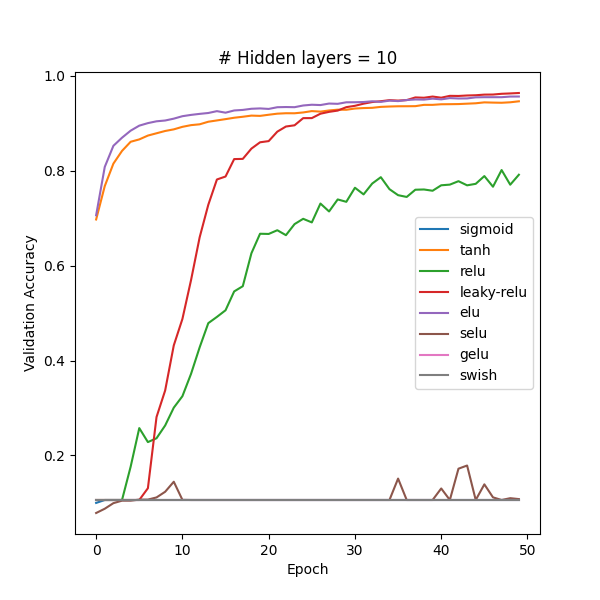
\includegraphics[width=0.4\textwidth]{images/10_hidden_layers_acc.png}
        }%
        \subfigure[Giá trị mất mát tập kiểm định (10)]{%
            \label{fig:mnistd3f}
            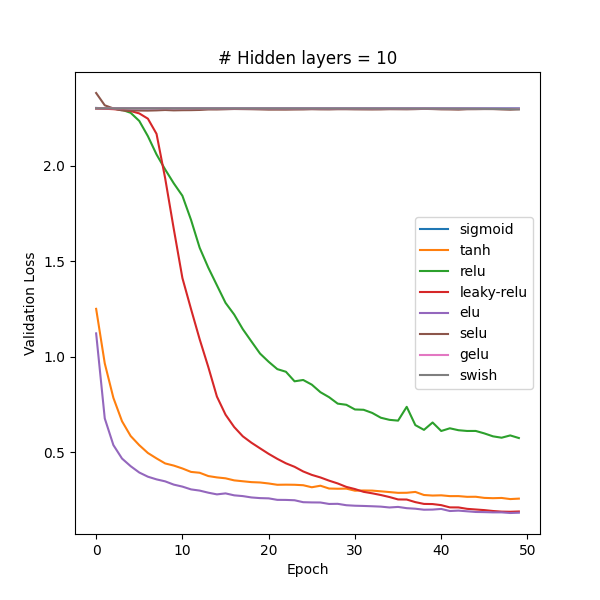
\includegraphics[width=0.4\textwidth]{images/10_hidden_layers_loss.png}
        }%
%
    \end{center}
    \caption{%
        Giá trị chính xác và mất mát (chuẩn hoá Lecun) trên tập kiểm định (số tầng ẩn: 8, 9, 10).
     }%
   \label{fig:mnistd3}
\end{figure}

\begin{figure}[ht!]
     \begin{center}
%
        \subfigure[Giá trị chính xác tập kiểm định (11)]{%
            \label{fig:mnistd4a}
            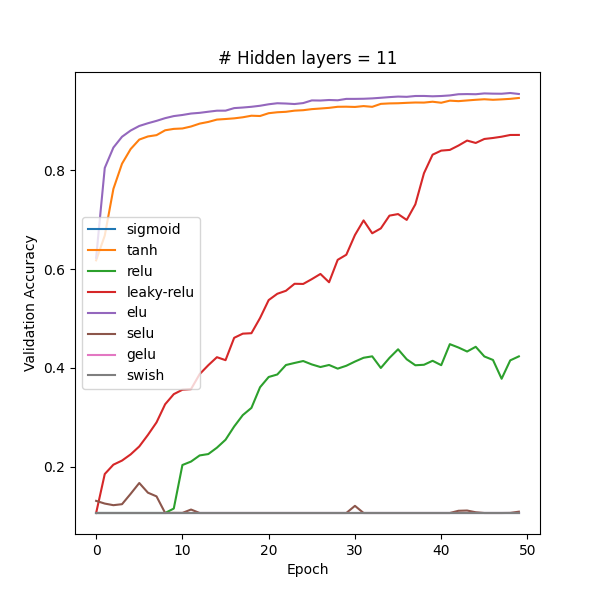
\includegraphics[width=0.4\textwidth]{images/11_hidden_layers_acc.png}
        }%
        \subfigure[Giá trị mất mát tập kiểm định (11)]{%
           \label{fig:mnistd4b}
           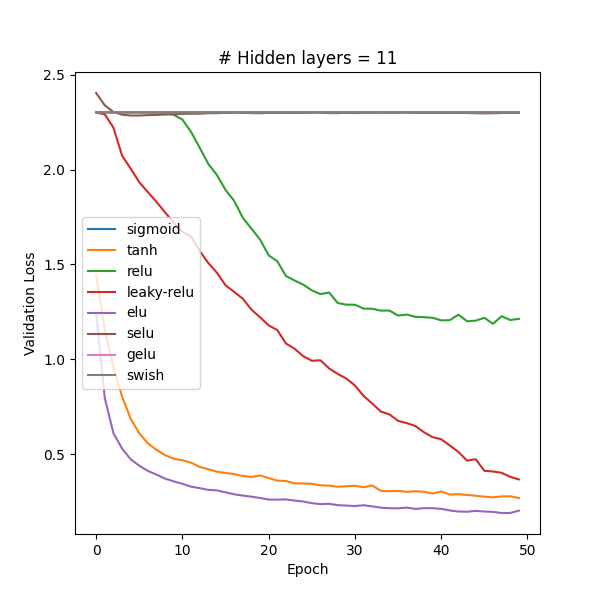
\includegraphics[width=0.4\textwidth]{images/11_hidden_layers_loss.png}
        }\\ %  ------- End of the first row ----------------------%
        \subfigure[Giá trị chính xác tập kiểm định (12)]{%
            \label{fig:mnistd4c}
            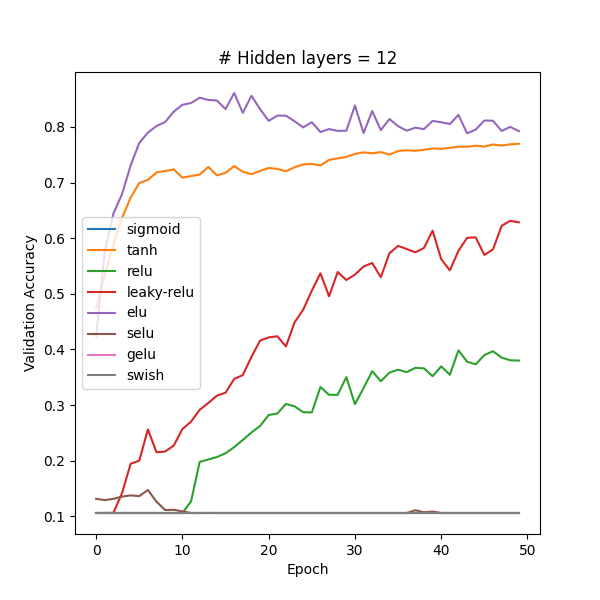
\includegraphics[width=0.4\textwidth]{images/12_hidden_layers_acc.png}
        }%
        \subfigure[Giá trị mất mát tập kiểm định (12)]{%
            \label{fig:mnistd4d}
            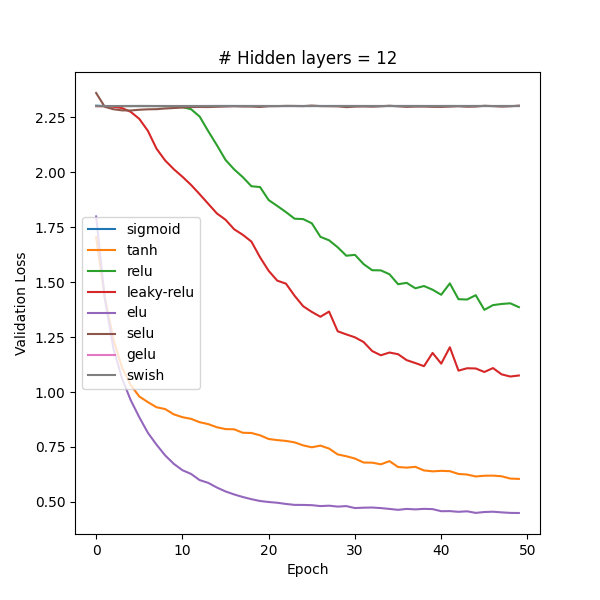
\includegraphics[width=0.4\textwidth]{images/12_hidden_layers_loss.png}
        }\\
        \subfigure[Giá trị chính xác so với số tầng ẩn]{%
            \label{fig:mnistd4e}
            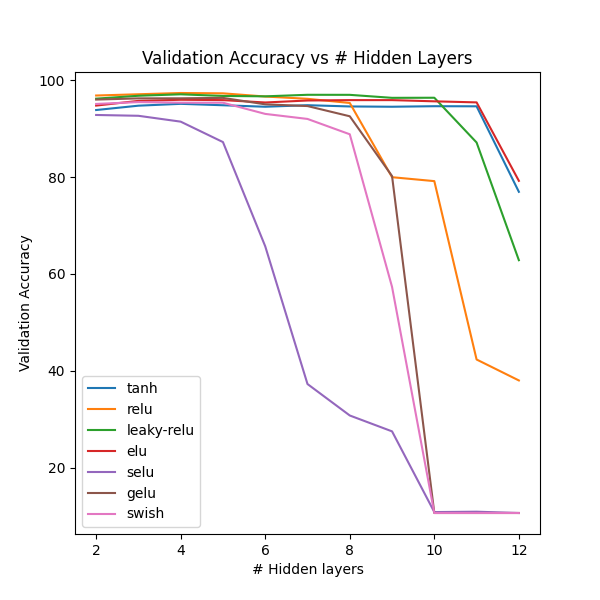
\includegraphics[width=0.4\textwidth]{images/vs_acc_hiddenlayers.png}
        }%
        \subfigure[Giá trị mất mát so với số tầng ẩn]{%
           \label{fig:mnistd4f}
           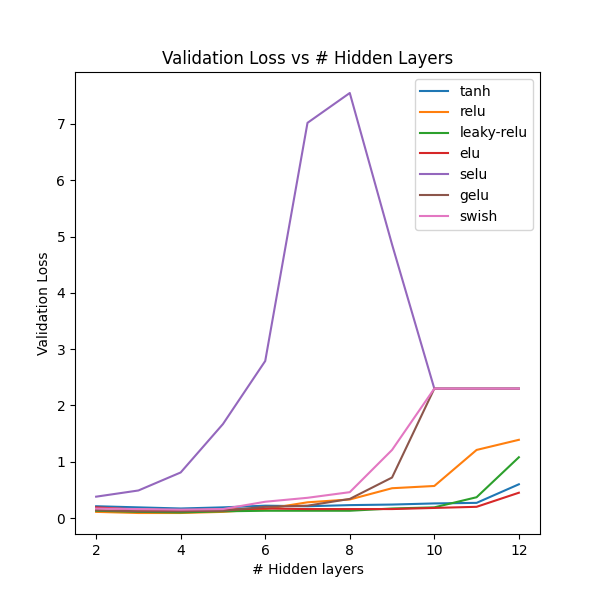
\includegraphics[width=0.4\textwidth]{images/vs_loss_hiddenlayers.png}
        }
%
    \end{center}
    \caption{%
        Giá trị chính xác và mất mát (chuẩn hoá Lecun) trên tập kiểm định (số tầng ẩn: 11, 12) [(a) - (d)]; Giá trị chính xác và mất mát (chuẩn hoá Lecun) trên tập kiểm định so với số tầng ẩn [(e), (f)].
     }%
   \label{fig:mnistd4}
\end{figure}

\clearpage

\subsection{Dữ liệu nhiễu Gauss và khởi tạo trọng số theo chuẩn hoá Lecun}\label{subsec:mnistnoise}

Dữ liệu bây giờ được tạo nhiễu theo hàm Gauss có độ lệch chuẩn $\sigma = 0.2$.
Hình \ref{fig:mnistexamplerawandnoise} cho ta thấy sự khác biệt giữa mẫu nguyên thuỷ và mẫu khi có nhiễu tác động vào.
Khoảng giá trị bây giờ của các phần tử trong mẫu nhiễu có thể âm (tức < 0) và cũng có thể lơn hơn 1.
Như trong ảnh \ref{fig:mnist5noise} có phần tử điểm ảnh có giá trị nhỏ nhất và lớn nhất lần lượt là $-0.5876574$ và $1.4352913$.

\begin{figure}[ht!]
     \begin{center}
%
        \subfigure[Ảnh chữ số 5 trong tập dữ liệu MNIST]{%
            \label{fig:mnist5raw}
            
\includegraphics[width=0.4\textwidth]{images/mnistraw.png}
        }%
        \subfigure[Ảnh chữ số 5 khi thêm nhiễu Gauss $\left(\sigma = 0.2\right)$ trong tập dữ liệu MNIST]{%
          \label{fig:mnist5noise}
          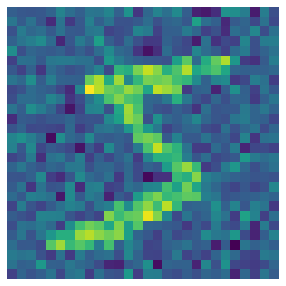
\includegraphics[width=0.4\textwidth]{images/mnistnoise.png}
        }
%
    \end{center}
    \caption{%
        Ví dụ về ảnh trước và sau khi thêm nhiễu Gauss từ tập dữ liệu MNIST.
     }%
  \label{fig:mnistexamplerawandnoise}
\end{figure}

Cách thức huấn luyện vẫn được áp dụng như phần \ref{subsec:mnistd}, tuy nhiên lần này có một chút khác biệt là kỹ thuật alpha dropout sẽ không được áp dụng cho SELU mà sẽ sử dụng cách dropout bình thường với cùng tỷ lệ như các hàm kích hoạt khác.
Biểu đồ giá trị chính xác và mất mát trên tập kiểm định qua mỗi epoch được cho ở các hình \ref{fig:mnistnoise1}, \ref{fig:mnistnoise2}, \ref{fig:mnistnoise3}, \ref{fig:mnistnoise4}.
Chi tiết về giá trị được cho ở bảng \ref{tab:mnistnoiseacc} và bảng \ref{tab:mnistnoiseloss}.

\begin{table}[ht!]
\centering
\def\arraystretch{1.1}
\begin{tabular}{c|c|c|c|c|c|c|c|c|c|c|c|}
\cline{2-12}
                        & 2     & 3     & 4     & 5     & 6     & 7     & 8     & 9     & 10    & 11    & 12    \\ \hline
\multicolumn{1}{|c|}{$\tanh$} & 92.14 & 93.10 & 93.40 & 93.09 & 92.83 & 93.35 & 92.98 & 92.74 & 92.86 & 92.13 & 67.80 \\ \hline
\multicolumn{1}{|c|}{$\mathcal{R}$} & \textbf{95.46} & \textbf{95.88} & \textbf{95.97} & \textbf{95.78} & 94.57 & 93.83 & 91.21 & 86.59 & 42.95 & 40.26 & 45.08 \\ \hline
\multicolumn{1}{|c|}{$\mathcal{R}_L$} & 94.83 & 95.18 & 95.55 & 95.14 & \textbf{94.63} & \textbf{95.04} & \textbf{95.10} & \textbf{94.01} & 93.08 & 73.42 & 54.34 \\ \hline
\multicolumn{1}{|c|}{$\mathcal{E}$} & 93.03 & 94.23 & 94.52 & 94.43 & 93.86 & 94.30 & 94.13 & 93.99 & 93.98 & \textbf{93.94} & \textbf{84.06} \\ \hline
\multicolumn{1}{|c|}{$\mathcal{E}_S$} & 91.46 & 93.10 & 93.76 & 93.66 & 93.32 & 94.12 & 94.31 & 93.06 & \textbf{94.03} & 93.77 & 68.40 \\ \hline
\multicolumn{1}{|c|}{$\mathcal{G}$} & 95.02 & 95.38 & 95.48 & 95.17 & 93.31 & 93.55 & 87.75 & 70.12 & 10.60 & 10.60 & 10.60 \\ \hline
\multicolumn{1}{|c|}{$\mathcal{S}$} & 94.08 & 94.42 & 94.42 & 94.02 & 92.34 & 88.00 & 80.94 & 46.26 & 21.84 & 10.60 & 10.60 \\ \hline
\end{tabular}
\caption{Giá trị chính xác (\%) của các hàm kích hoạt (nhiễu Gauss + chuẩn hoá Lecun) tương ứng với các số tầng ẩn của mô hình trên tập dữ liệu MNIST.}
\label{tab:mnistnoiseacc}
\end{table}

\begin{table}[ht!]
\centering
\def\arraystretch{1.3}
\begin{tabular}{c|c|c|c|c|c|c|c|c|c|c|c|}
\cline{2-12}
                        & 2    & 3    & 4    & 5    & 6    & 7    & 8    & 9    & 10   & 11   & 12   \\ \hline
\multicolumn{1}{|c|}{$\tanh$} & 0.26 & 0.23 & 0.22 & 0.25 & 0.28 & 0.28 & 0.30 & 0.31 & 0.34 & 0.37 & 0.77 \\ \hline
\multicolumn{1}{|c|}{$\mathcal{R}$} & \textbf{0.15} & \textbf{0.13} & \textbf{0.15} & \textbf{0.17} & 0.31 & 0.36 & 0.49 & 0.59 & 1.35 & 1.30 & 1.48 \\ \hline
\multicolumn{1}{|c|}{$\mathcal{R}_L$} & 0.17 & 0.15 & 0.16 & \textbf{0.17} & \textbf{0.23} & \textbf{0.21} & \textbf{0.22} & 0.34 & 0.38 & 0.78 & 1.24 \\ \hline
\multicolumn{1}{|c|}{$\mathcal{E}$} & 0.23 & 0.19 & 0.18 & 0.19 & \textbf{0.23} & \textbf{0.21} & \textbf{0.22} & \textbf{0.24} & \textbf{0.25} & \textbf{0.27} & \textbf{0.51} \\ \hline
\multicolumn{1}{|c|}{$\mathcal{E}_S$} & 0.29 & 0.24 & 0.21 & 0.21 & 0.24 & 0.23 & 0.23 & 0.25 & 0.26 & 0.28 & 0.72 \\ \hline
\multicolumn{1}{|c|}{$\mathcal{G}$} & 0.16 & 0.15 & \textbf{0.15} & \textbf{0.17} & 0.29 & 0.28 & 0.57 & 0.94 & 2.30 & 2.30 & 2.30 \\ \hline
\multicolumn{1}{|c|}{$\mathcal{S}$} & 0.20 & 0.18 & 0.19 & 0.21 & 0.30 & 0.48 & 0.65 & 1.50 & 2.02 & 2.30 & 2.30 \\ \hline
\end{tabular}
\caption{Giá trị mất mát của các hàm kích hoạt (nhiễu Gauss + chuẩn hoá Lecun) tương ứng với các mô hình trên tập dữ liệu MNIST.}
\label{tab:mnistnoiseloss}
\end{table}

Ở những kiến trúc đầu tiên, chẳng hạn khi độ sâu tầng ẩn là 2 (hình \ref{fig:mnistnoise1a}, \ref{fig:mnistnoise1a}), chưa có sự phân hoá rõ ràng giữa các hàm.
Nếu tính chi ly, thì ta có 2 cái tên quen thuộc ở những lượt đầu là RELU và Leaky có độ chính xác cao nhất (95.46\% và 94.83\%).
Trong nhóm có độ chính xác $\approx$ 95\% thì có GELU (95.02\%) - hàm không cho kết quả không khả quan ở phần thực nghiệm trước (phần \ref{subsec:mnistd}).
\vspace{5pt}

Khi số tầng ẩn đã là 5 (hình \ref{fig:mnistnoise2a}, \ref{fig:mnistnoise2a}), chất lượng độ chính xác của các hàm kích hoạt vẫn chưa phân nhóm khi tất cả đều xấp xỉ khoảng 94-95\%.
Hàm Tanh có tốc độ hội tụ khá nhanh khi chỉ cần 15 epoch để đạt ngưỡng (bảng \ref{tab:mnistnoiseepoch}).
Dẫu vậy, rõ ràng là nhận định hàm Tanh tìm được hố cực tiểu nông là một nhận định hợp lý khi sau 50 epoch, giá trị mất mát của hàm này không thay đổi nhiều và đứng ở 0.25, trở thành hàm có mất mát cao nhất trong lượt này.

\begin{table}[ht!]
\centering
\def\arraystretch{1.3}
\begin{tabular}{c|c|c|c|c|c|c|c|c|c|c|c|c|}
\cline{2-13}
                        & 2  & 3  & 4  & 5  & 6  & 7  & 8  & 9  & 10 & 11 & 12 & $\mu$ \\ \hline
\multicolumn{1}{|c|}{$\tanh$} & 10 & 20 & \textbf{20} & \textbf{15} & 19 & \textbf{23} & \textbf{16} & \textbf{22} & 24 & 31 & 15 & \textbf{20}\\ \hline
\multicolumn{1}{|c|}{$\mathcal{R}$} & 29 & 31 & 24 & 27 & 29 & 36 & 33 & 41 & \textbf{18} & 26 & 16 & 28\\ \hline
\multicolumn{1}{|c|}{$\mathcal{R}_L$} & 29 & 30 & 26 & 27 & 28 & 26 & 28 & 29 & 40 & 35 & 30 & 30\\ \hline
\multicolumn{1}{|c|}{$\mathcal{E}$} & 20 & 29 & 29 & 27 & 25 & 25 & 25 & 25 & 28 & \textbf{23} & 30 & 26\\ \hline
\multicolumn{1}{|c|}{$\mathcal{E}_S$} & \textbf{4}  & \textbf{16} & 22 & 22 & \textbf{18} & \textbf{23} & 22 & \textbf{22} & 24 & 26 & \textbf{9}  & \textbf{20}\\ \hline
\multicolumn{1}{|c|}{$\mathcal{G}$} & 34 & 33 & 33 & 32 & 38 & 40 & 46 & 46 & 1  & 1  & 1  & X\\ \hline
\multicolumn{1}{|c|}{$\mathcal{S}$} & 31 & 33 & 31 & 33 & 39 & 39 & 44 & 41 & 1  & 1  & 1  & X\\ \hline
\end{tabular}
\caption{Số epoch cần thiết để 80\% giá trị mất mát (nhiễu Gauss + chuẩn hoá Lecun) bằng giá trị mất mát cuối cùng.}
\label{tab:mnistnoiseepoch}
\end{table}

Tới 7 tầng ẩn (hình \ref{fig:mnistnoise2e}, \ref{fig:mnistnoise2f}), Swish là cái tên đầu tiên có vẽ không còn đủ khả năng để đi tiếp.
Tuy RELU và GELU có màn thể hiện rất tốt ở gian đoạn đầu, nhưng cũng như lần thử nghiệm trước (phần \ref{subsec:mnistd}), khi số tầng ẩn khá sâu thì đã giảm hiệu quả của 2 hàm này.
Leaky tuy hội tụ khá chậm so với nhóm đầu - nhóm gồm Tanh, ELU và SELU khi phải mất tới 36 epoch mới đạt ngưỡng, nhưng về cuối lại có một kết quả chính xác tốt khi vẫn trên 90\% và cao hơn cả hàm Tanh (93.83\% > 92.92\%).
Một điểm khá bất ngờ là khi không áp dụng alpha dropout, SELU đạt kết quả rất tốt.
Không chỉ có giá trị chính xác cao, mất mát thấp mà việc hội tụ cũng rất nhanh khi đạt ngưỡng sau 23 epoch, ngang với hàm dễ đạt ngưỡng như Tanh.
\vspace{5pt}

Hình \ref{fig:mnistnoise3c} và hình \ref{fig:mnistnoise3d} cho thấy rằng GELU không còn có thể duy trì được phong độ như RELU đang làm.
Tuy là RELU có vẻ không phù hợp cho những mạng sâu, nhưng giá trị chính xác và mất mát không ở mức quá tệ (chính xác 86.59\% và mất mát 0.59).
Leaky giờ đây đã tụt xuống ngang với hàm Tanh, dẫn đến việc ta thấy Leaky hội tụ rất lâu, và phải tới 41 epoch mới đạt ngưỡng.
ELU và người anh em SELU của mình nổi trội với độ chính xác 94\% $\pm$ 0.01\%.
Ngoài ra 2 hàm trên, còn Tanh và Leaky là hai hàm có giá trị chính xác trên tập kiểm định trên 90\% sau 50 epoch.
Điều này được kéo dài và kết thúc ngay khi số tầng ẩn tăng lên 11 (hình \ref{fig:mnistnoise4a}, \ref{fig:mnistnoise4b}) khi giá trị chính xác Leaky lúc này chỉ còn 73.42\%, trong khi 3 hàm Tanh, ELU và SELU vẫn trên 90\%.
\vspace{5pt}

Ở kiến trúc cuối cùng - 12 tầng ẩn (hình \ref{fig:mnistnoise4c}, \ref{fig:mnistnoise4d}), có 3 nhóm tách biệt khá rõ rệt (không tính những hàm không còn khả năng học là GELU và Swish).
Nhóm kết quả thấp nhất là RELU và Leaky với độ chính xác tầm khoảng 50\% (45.05\% và 54.34\%) và mất mát cao hơn 1.0 (1.48 và 1.24).
Nhóm giữa là Tanh và SELU với mất mát xấp xỉ nhau với mất mát là 0.77 và 0.72, giá trị chính xác của cả hai $\approx$ 68\%.
Nhóm có kết quả tốt nhất và cũng chỉ duy nhất ELU khi giá trị chính xác là 84.06\% (vẫn trên 80\%).

\begin{table}[ht!]
\centering
\def\arraystretch{1.5}
\begin{tabular}{c|c|c|c|c|c|c|c|}
\cline{2-8}
                        & $\tanh$      & $\mathcal{R}$      & $\mathcal{R}_L$      & $\mathcal{E}$      & $\mathcal{E}_S$      & $\mathcal{G}$      & $\mathcal{S}$      \\ \hline
\multicolumn{1}{|c|}{$\mu_{\text{chính xác}}$ (\%)} & 90.58  & 79.78  & 89.12  & \textbf{93.13}  & 91.27  & 68.87  & 66.14  \\ \hline
\multicolumn{1}{|c|}{$\sigma^2_{\text{chính xác}} (\%)$} & 0.0052 & 0.0522 & 0.0159 & \textbf{0.0008} & 0.0053 & 0.1321 & 0.1188 \\ \hline
\multicolumn{1}{|c|}{$\mu_{\text{mất mát}}$} & 0.33   & 0.59   & 0.37   & \textbf{0.25}   & 0.29   & 0.88   & 0.94   \\ \hline
\multicolumn{1}{|c|}{$\sigma^2_{\text{mất mát}}$} & 0.0215 & 0.2526 & 0.1068 & \textbf{0.0072} & 0.0194 & 0.8121 & 0.7380 \\ \hline
\end{tabular}
\caption{Giá trị trung bình và phương sai của các hàm kích hoạt (nhiễu Gauss + chuẩn hoá Lecun) trong 11 mô hình thử nghiệm.}
\label{tab:mnistnoisemean}
\end{table}

Kết quả của lần thực nghiệm này không có quá nhiều khác biệt (hình \ref{fig:mnistnoise4e}, \ref{fig:mnistnoise4f}) so với lần thử nghiệm khi tập dữ liệu không có nhiễu (phần \ref{subsec:mnistd}).
Hàm RELU và Leaky vẫn là những hàm nổi trội với giá trị chính xác cao trong những mô hình có độ sâu vừa phải.
Về hàm Tanh, vẫn là một hàm không thể hiện được sức mạnh ở những mô hình đầu như RELU hay Leaky khi nhanh chóng tìm một hố sâu cực tiểu.
Tuy vậy, điều này lại vẫn là lợi thế khi tầng ẩn trong các mạng được nâng lên, đó là lí do mà Tanh có $\mu_{\text{chính xác}} = 90.58\%$ sau 11 mô hình.
ELU vẫn là hàm có kết quả tốt nhất với $\mu_{\text{chính xác}} = 93.13\%$ và $\mu_{\text{mất mát}} = 0.25$.
SELU cũng có kết quả rất khả quan sau khi loại bỏ đi kỷ thuật alpha dropout cho mô hình có hàm kích hoạt này khi có $\mu_{\text{chính xác}} = 91.27\%$ (chỉ thua mỗi ELU).
Một ấn tượng nữa của SELU là nó cũng có tốc độ hội tụ khá nhanh, ngang tới Tanh.
Dẫu thế, vẫn chưa khẳng định là SELU cũng chỉ tìm hố cực tiểu nông như Tanh vì ngoại trừ 12 tầng ẩn, những mô hình còn lại SELU có giá trị mất mát cách một hàm cho kết quả tốt như ELU không quá 0.03.

\begin{figure}[ht!]
     \begin{center}
%
        \subfigure[Giá trị chính xác tập kiểm định (2)]{%
            \label{fig:mnistnoise1a}
            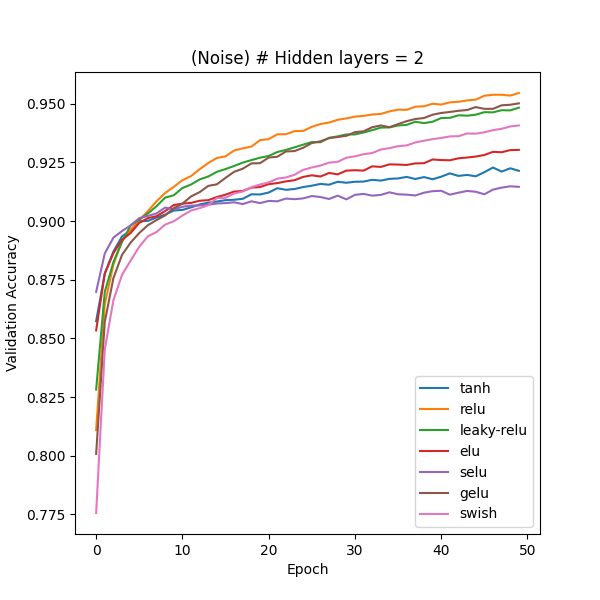
\includegraphics[width=0.4\textwidth]{images/noise_2_hidden_layers_acc.png}
        }%
        \subfigure[Giá trị mất mát tập kiểm định (2)]{%
          \label{fig:mnistnoise1b}
          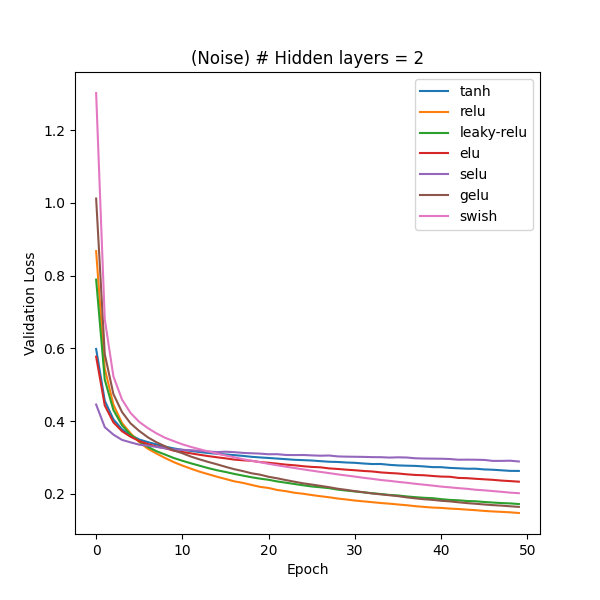
\includegraphics[width=0.4\textwidth]{images/noise_2_hidden_layers_loss.png}
        }\\ %  ------- End of the first row ----------------------%
        \subfigure[Giá trị chính xác tập kiểm định (3)]{%
            \label{fig:mnistnoise1c}
            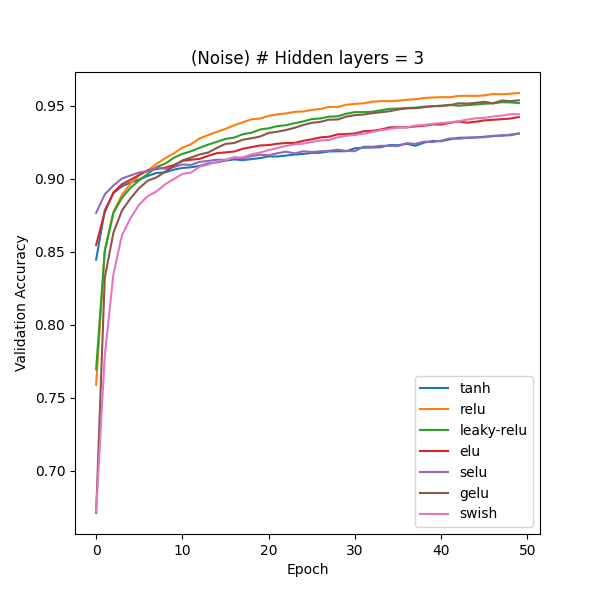
\includegraphics[width=0.4\textwidth]{images/noise_3_hidden_layers_acc.png}
        }%
        \subfigure[Giá trị mất mát tập kiểm định (3)]{%
            \label{fig:mnistnoise1d}
            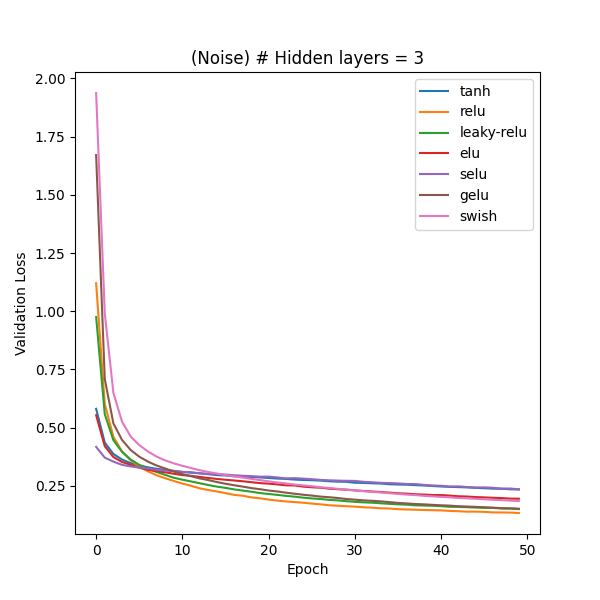
\includegraphics[width=0.4\textwidth]{images/noise_3_hidden_layers_loss.png}
        }\\
        %----------------------%
        \subfigure[Giá trị chính xác tập kiểm định (4)]{%
            \label{fig:mnistnoise1e}
            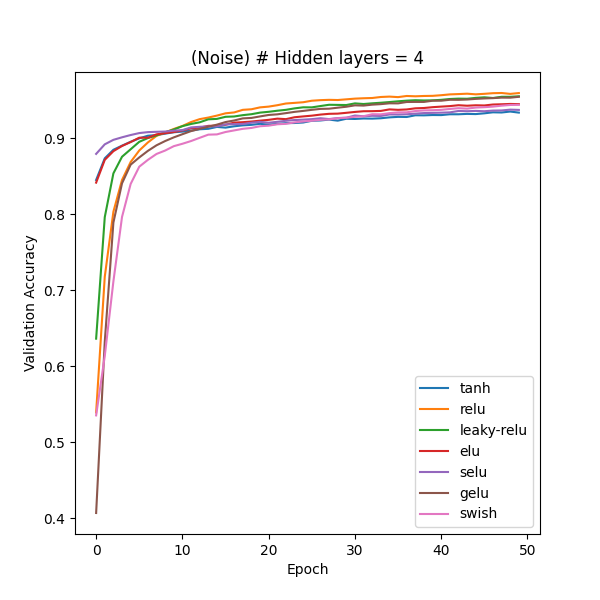
\includegraphics[width=0.4\textwidth]{images/noise_4_hidden_layers_acc.png}
        }%
        \subfigure[Giá trị mất mát tập kiểm định (4)]{%
            \label{fig:mnistnoise1f}
            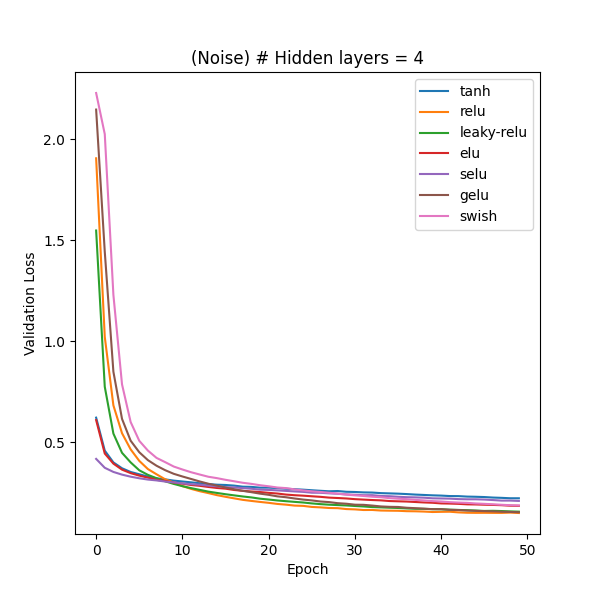
\includegraphics[width=0.4\textwidth]{images/noise_4_hidden_layers_loss.png}
        }%
%
    \end{center}
    \caption{%
        Giá trị chính xác và mất mát (nhiễu Gauss + chuẩn hoá Lecun) trên tập kiểm định (số tầng ẩn: 2, 3, 4).
     }%
  \label{fig:mnistnoise1}
\end{figure}

\begin{figure}[ht!]
     \begin{center}
%
        \subfigure[Giá trị chính xác tập kiểm định (5)]{%
            \label{fig:mnistnoise2a}
            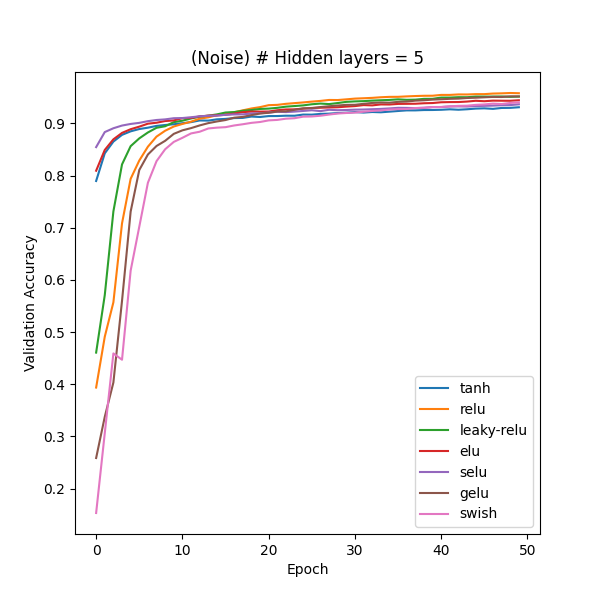
\includegraphics[width=0.4\textwidth]{images/noise_5_hidden_layers_acc.png}
        }%
        \subfigure[Giá trị mất mát tập kiểm định (5)]{%
          \label{fig:mnistnoise2b}
          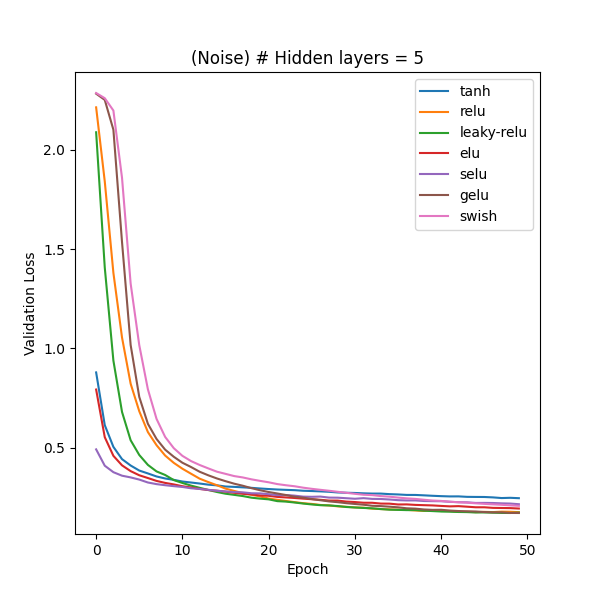
\includegraphics[width=0.4\textwidth]{images/noise_5_hidden_layers_loss.png}
        }\\ %  ------- End of the first row ----------------------%
        \subfigure[Giá trị chính xác tập kiểm định (6)]{%
            \label{fig:mnistnoise2c}
            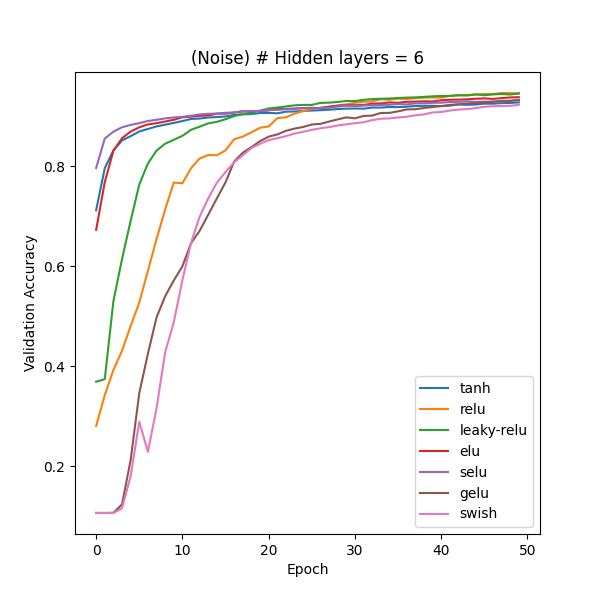
\includegraphics[width=0.4\textwidth]{images/noise_6_hidden_layers_acc.png}
        }%
        \subfigure[Giá trị mất mát tập kiểm định (6)]{%
            \label{fig:mnistnoise2d}
            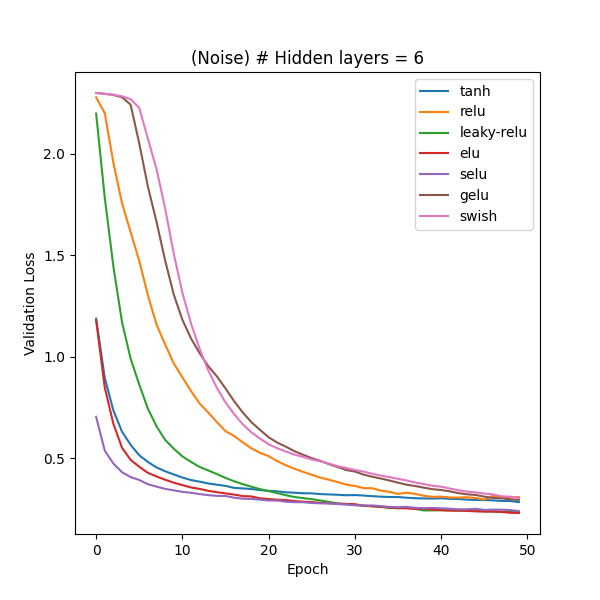
\includegraphics[width=0.4\textwidth]{images/noise_6_hidden_layers_loss.png}
        }\\
        %----------------------%
        \subfigure[Giá trị chính xác tập kiểm định (7)]{%
            \label{fig:mnistnoise2e}
            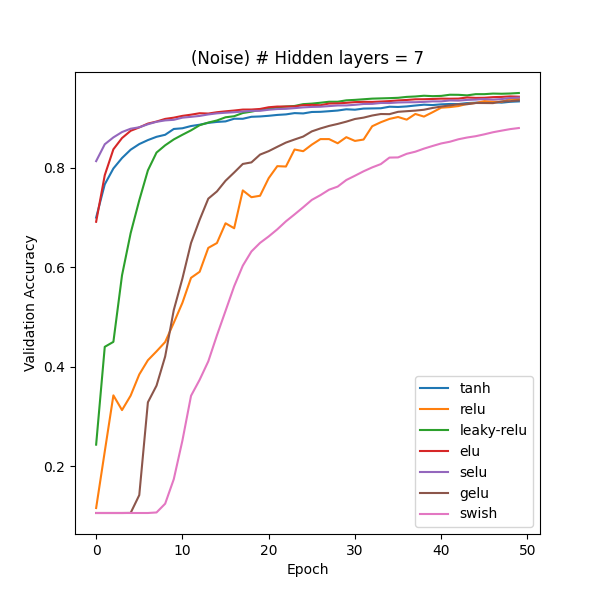
\includegraphics[width=0.4\textwidth]{images/noise_7_hidden_layers_acc.png}
        }%
        \subfigure[Giá trị mất mát tập kiểm định (7)]{%
            \label{fig:mnistnoise2f}
            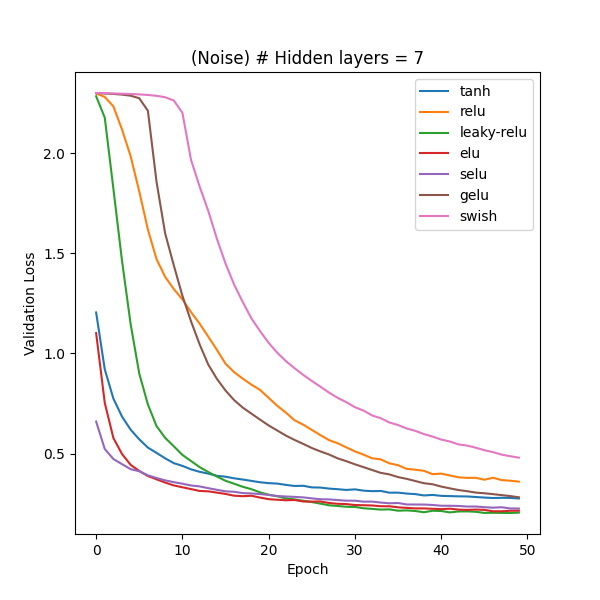
\includegraphics[width=0.4\textwidth]{images/noise_7_hidden_layers_loss.png}
        }%
%
    \end{center}
    \caption{%
        Giá trị chính xác và mất mát (nhiễu Gauss + chuẩn hoá Lecun) trên tập kiểm định (số tầng ẩn: 5, 6, 7).
     }%
  \label{fig:mnistnoise2}
\end{figure}

\begin{figure}[ht!]
     \begin{center}
%
        \subfigure[Giá trị chính xác tập kiểm định (8)]{%
            \label{fig:mnistnoise3a}
            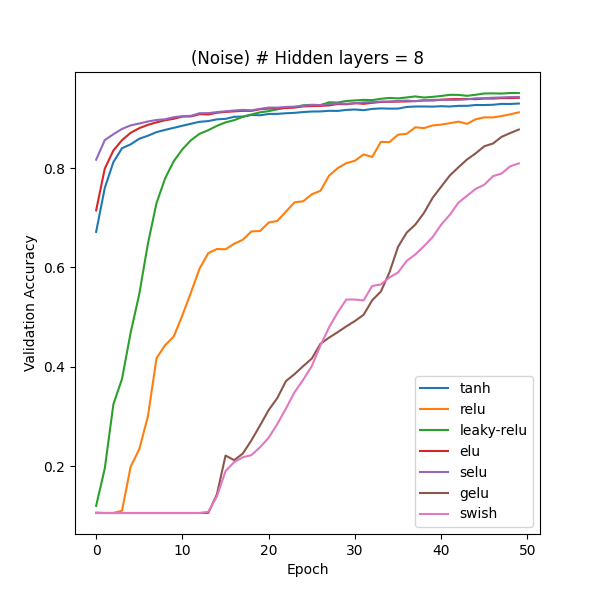
\includegraphics[width=0.4\textwidth]{images/noise_8_hidden_layers_acc.png}
        }%
        \subfigure[Giá trị mất mát tập kiểm định (8)]{%
          \label{fig:mnistnoise3b}
          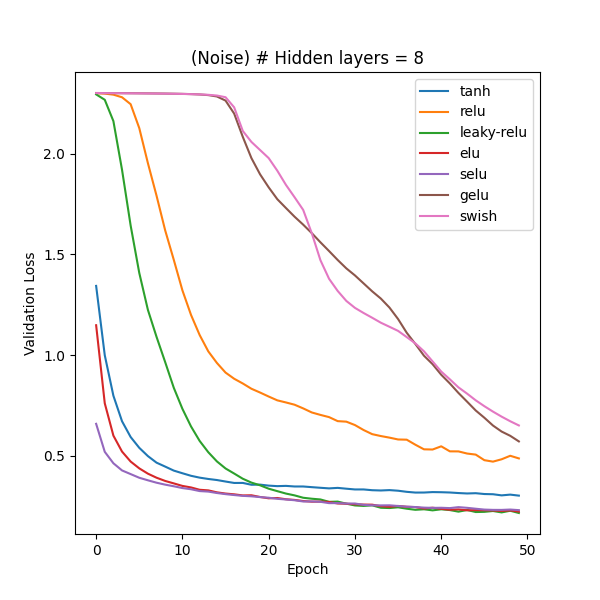
\includegraphics[width=0.4\textwidth]{images/noise_8_hidden_layers_loss.png}
        }\\ %  ------- End of the first row ----------------------%
        \subfigure[Giá trị chính xác tập kiểm định (9)]{%
            \label{fig:mnistnoise3c}
            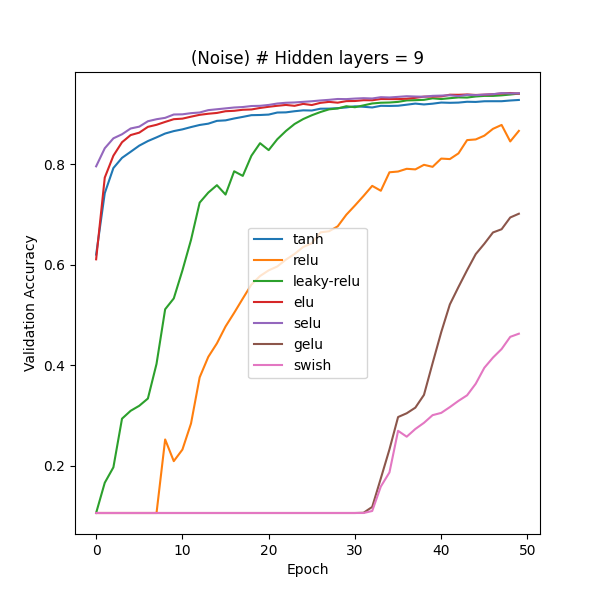
\includegraphics[width=0.4\textwidth]{images/noise_9_hidden_layers_acc.png}
        }%
        \subfigure[Giá trị mất mát tập kiểm định (9)]{%
            \label{fig:mnistnoise3d}
            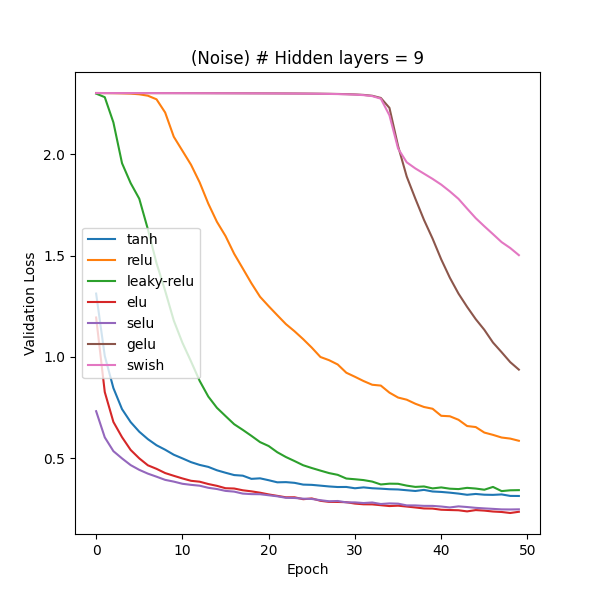
\includegraphics[width=0.4\textwidth]{images/noise_9_hidden_layers_loss.png}
        }\\
        %----------------------%
        \subfigure[Giá trị chính xác tập kiểm định (10)]{%
            \label{fig:mnistnoise3e}
            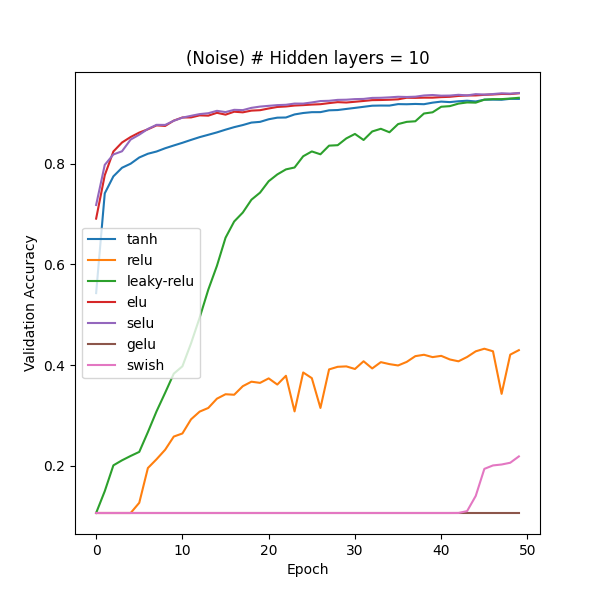
\includegraphics[width=0.4\textwidth]{images/noise_10_hidden_layers_acc.png}
        }%
        \subfigure[Giá trị mất mát tập kiểm định (10)]{%
            \label{fig:mnistnoise3f}
            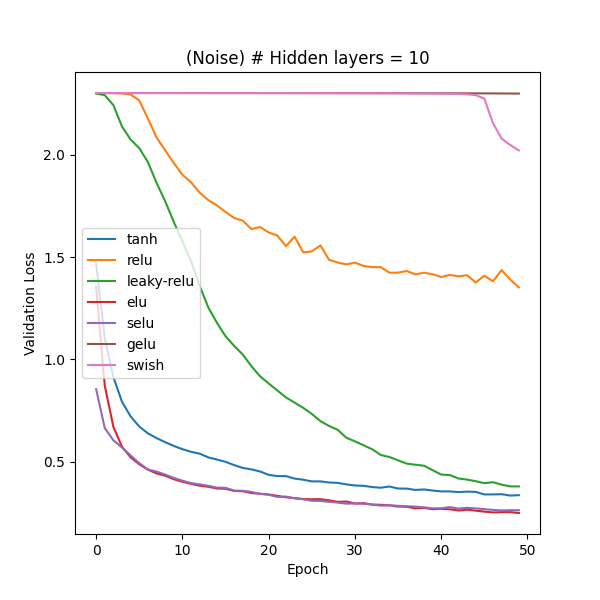
\includegraphics[width=0.4\textwidth]{images/noise_10_hidden_layers_loss.png}
        }%
%
    \end{center}
    \caption{%
        Giá trị chính xác và mất mát (nhiễu Gauss + chuẩn hoá Lecun) trên tập kiểm định (số tầng ẩn: 8, 9, 10).
     }%
  \label{fig:mnistnoise3}
\end{figure}

\begin{figure}[ht!]
     \begin{center}
%
        \subfigure[Giá trị chính xác tập kiểm định (11)]{%
            \label{fig:mnistnoise4a}
            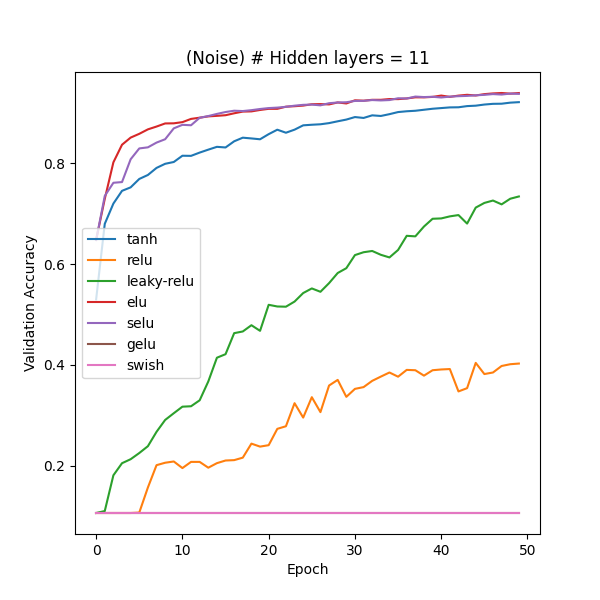
\includegraphics[width=0.4\textwidth]{images/noise_11_hidden_layers_acc.png}
        }%
        \subfigure[Giá trị mất mát tập kiểm định (11)]{%
          \label{fig:mnistnoise4b}
          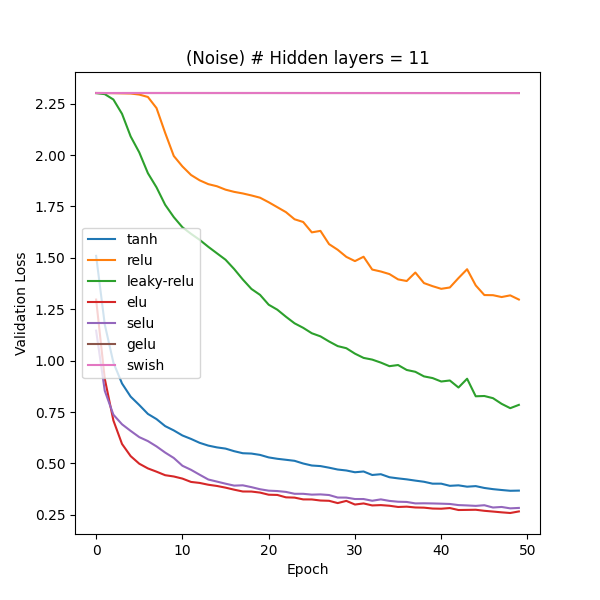
\includegraphics[width=0.4\textwidth]{images/noise_11_hidden_layers_loss.png}
        }\\ %  ------- End of the first row ----------------------%
        \subfigure[Giá trị chính xác tập kiểm định (12)]{%
            \label{fig:mnistnoise4c}
            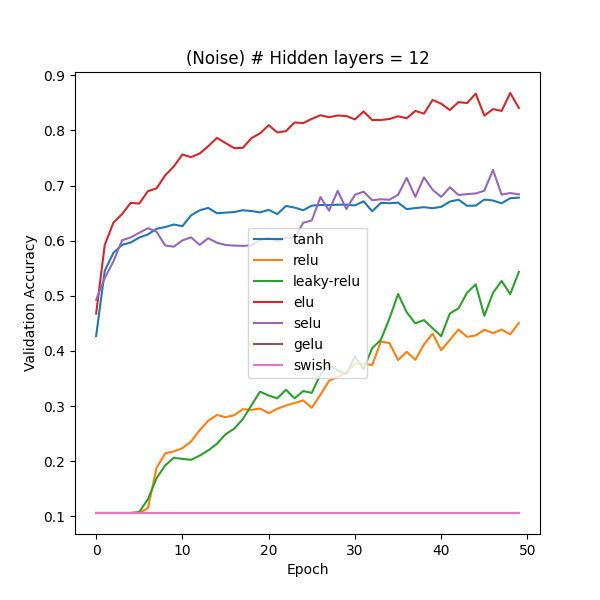
\includegraphics[width=0.4\textwidth]{images/noise_12_hidden_layers_acc.png}
        }%
        \subfigure[Giá trị mất mát tập kiểm định (12)]{%
            \label{fig:mnistnoise4d}
            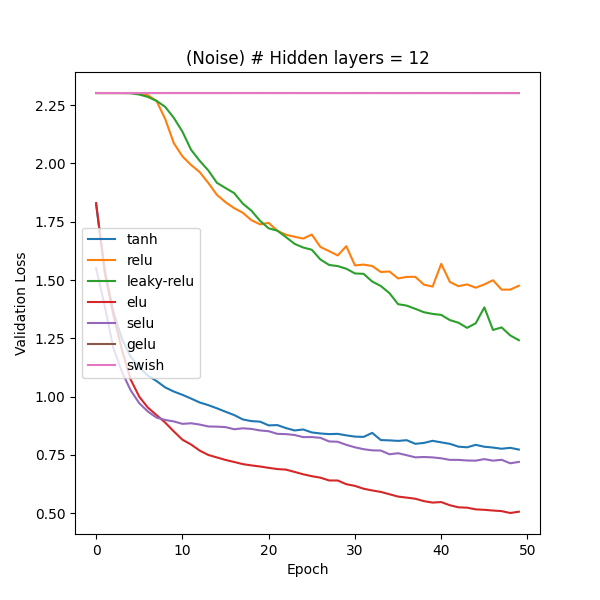
\includegraphics[width=0.4\textwidth]{images/noise_12_hidden_layers_loss.png}
        }\\
        \subfigure[Giá trị chính xác so với số tầng ẩn]{%
            \label{fig:mnistnoise4e}
            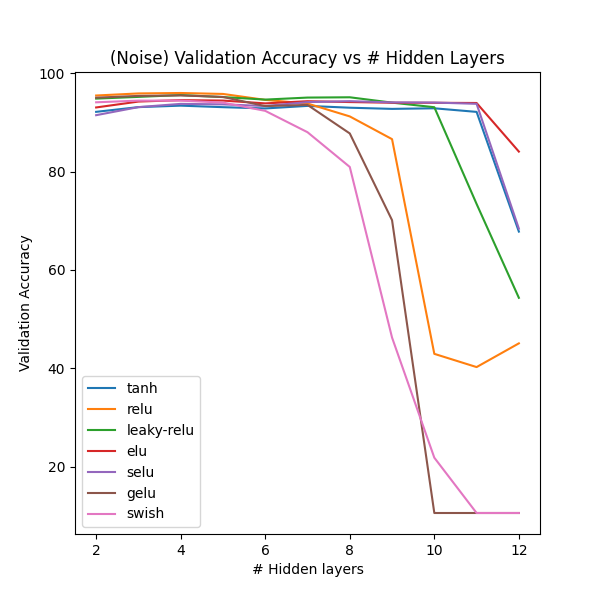
\includegraphics[width=0.4\textwidth]{images/vs_noise_acc_hiddenlayers.png}
        }%
        \subfigure[Giá trị mất mát so với số tầng ẩn]{%
          \label{fig:mnistnoise4f}
          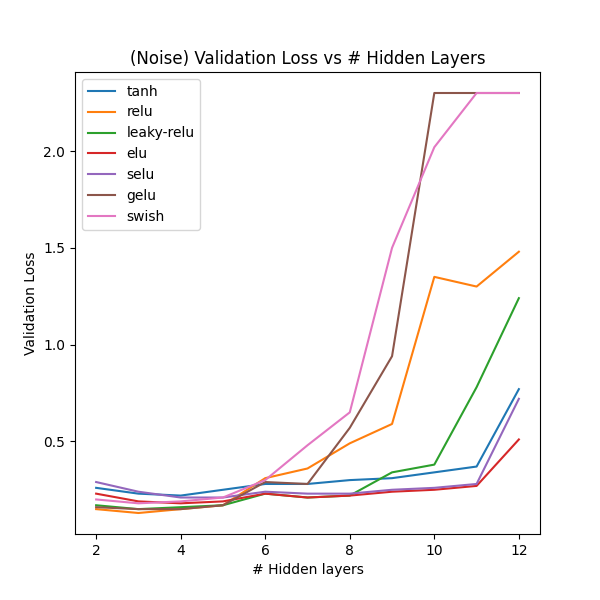
\includegraphics[width=0.4\textwidth]{images/vs_noise_loss_hiddenlayers.png}
        }
%
    \end{center}
    \caption{%
        Giá trị chính xác và mất mát (nhiễu Gauss + chuẩn hoá Lecun) trên tập kiểm định (số tầng ẩn: 11, 12) [(a) - (d)]; Giá trị chính xác và mất mát (nhiễu Gauss + chuẩn hoá Lecun) trên tập kiểm định so với số tầng ẩn [(e), (f)].
     }%
  \label{fig:mnistnoise4}
\end{figure}

\clearpage

\subsection{Dữ liệu nhiễu và không sử dụng kỹ thuật khởi tạo trọng số}\label{subsec:mnistwowinoise}

Quá trình thực nghiệm lần này gần như không thay đổi so với phần \ref{subsec:mnistnoise}, chỉ có một thay đổi nhỏ đó là không khởi tạo trọng số bằng chuẩn Lecun mà sẽ để ngẫu nhiên.
Biểu đồ giá trị chính xác và mất mát trên tập kiểm định qua mỗi epoch được cho ở các hình \ref{fig:wowinoise1}, \ref{fig:wowinoise2}, \ref{fig:wowinoise3}, \ref{fig:wowinoise4}.
Chi tiết về giá trị được cho ở bảng \ref{tab:wowinoiseacc} và bảng \ref{tab:wowinoiseloss}.

\begin{table}[ht!]
\centering
\def\arraystretch{1.1}
\begin{tabular}{c|c|c|c|c|c|c|c|c|c|c|c|}
\cline{2-12}
                        & 2     & 3     & 4     & 5     & 6     & 7     & 8     & 9     & 10    & 11    & 12    \\ \hline
\multicolumn{1}{|c|}{$\tanh$} & 92.47 & 93.17 & 93.57 & 93.38 & 92.98 & 93.27 & 93.03 & 93.04 & 92.73 & 91.93 & 84.08 \\ \hline
\multicolumn{1}{|c|}{$\mathcal{R}$} & \textbf{95.35} & \textbf{95.74} & \textbf{95.94} & \textbf{95.72} & 94.03 & 90.69 & 92.37 & 90.34 & 76.84 & 38.36 & 31.90 \\ \hline
\multicolumn{1}{|c|}{$\mathcal{R}_L$} & 94.67 & 95.42 & 95.20 & 95.46 & \textbf{94.93} & \textbf{95.20} & \textbf{95.07} & \textbf{94.90} & 93.56 & 89.71 & 73.43 \\ \hline
\multicolumn{1}{|c|}{$\mathcal{E}$} & 92.32 & 94.23 & 94.51 & 94.31 & 93.94 & 94.32 & 94.71 & 94.35 & \textbf{94.05} & \textbf{93.95} & \textbf{86.58} \\ \hline
\multicolumn{1}{|c|}{$\mathcal{E}_S$} & 92.35 & 93.87 & 94.08 & 93.98 & 93.86 & 94.18 & 94.42 & 94.65 & 93.86 & 84.70 & 82.53 \\ \hline
\multicolumn{1}{|c|}{$\mathcal{G}$} & 95.03 & 95.45 & 95.48 & 95.47 & 93.61 & 94.07 & 93.18 & 90.57 & 83.99 & 46.11 & 10.60 \\ \hline
\multicolumn{1}{|c|}{$\mathcal{S}$} & 94.19 & 94.35 & 94.61 & 94.35 & 93.05 & 92.55 & 88.78 & 88.49 & 71.93 & 10.60 & 10.60 \\ \hline
\end{tabular}
\caption{Giá trị chính xác (\%) của các hàm kích hoạt (nhiễu) tương ứng với các số tầng ẩn của mô hình trên tập dữ liệu MNIST.}
\label{tab:wowinoiseacc}
\end{table}

\begin{table}[ht!]
\centering
\def\arraystretch{1.3}
\begin{tabular}{c|c|c|c|c|c|c|c|c|c|c|c|}
\cline{2-12}
                        & 2    & 3    & 4    & 5    & 6    & 7    & 8    & 9    & 10   & 11   & 12   \\ \hline
\multicolumn{1}{|c|}{$\tanh$} & 0.26 & 0.23 & 0.22 & 0.24 & 0.29 & 0.29 & 0.30 & 0.31 & 0.34 & 0.38 & 0.52 \\ \hline
\multicolumn{1}{|c|}{$\mathcal{R}$} & \textbf{0.15} & \textbf{0.14} & \textbf{0.15} & 0.18 & 0.33 & 0.42 & 0.48 & 0.55 & 0.87 & 1.43 & 1.5  \\ \hline
\multicolumn{1}{|c|}{$\mathcal{R}_L$} & 0.18 & 0.15 & 0.16 & 0.16 & \textbf{0.21} & \textbf{0.20} & 0.23 & 0.23 & 0.36 & 0.54 & 0.83 \\ \hline
\multicolumn{1}{|c|}{$\mathcal{E}$} & 0.23 & 0.19 & 0.18 & 0.19 & 0.22 & 0.21 & \textbf{0.22} & \textbf{0.23} & \textbf{0.25} & \textbf{0.26} & \textbf{0.46} \\ \hline
\multicolumn{1}{|c|}{$\mathcal{E}_S$} & 0.27 & 0.21 & 0.20 & 0.21 & 0.23 & 0.22 & 0.23 & 0.24 & 0.27 & 0.41 & 0.51 \\ \hline
\multicolumn{1}{|c|}{$\mathcal{G}$} & 0.16 & 0.15 & \textbf{0.15} & \textbf{0.16} & 0.27 & 0.24 & 0.31 & 0.40 & 0.58 & 1.53 & 2.30 \\ \hline
\multicolumn{1}{|c|}{$\mathcal{S}$} & 0.20 & 0.18 & 0.18 & 0.19 & 0.26 & 0.29 & 0.45 & 0.47 & 0.95 & 2.30 & 2.30 \\ \hline
\end{tabular}
\caption{Giá trị mất mát của các hàm kích hoạt (nhiễu) tương ứng với các mô hình trên tập dữ liệu MNIST.}
\label{tab:wowinoiseloss}
\end{table}

\begin{table}[ht!]
\centering
\def\arraystretch{1.3}
\begin{tabular}{c|c|c|c|c|c|c|c|c|c|c|c|c|}
\cline{2-13}
                        & 2  & 3  & 4  & 5  & 6  & 7  & 8  & 9  & 10 & 11 & 12 & $\mu$ \\ \hline
\multicolumn{1}{|c|}{$\tanh$} & 10 & \textbf{19} & \textbf{21} & 23 & \textbf{19} & \textbf{22} & \textbf{19} & \textbf{24} & 27 & 32 & 32 & 23\\ \hline
\multicolumn{1}{|c|}{$\mathcal{R}$} & 30 & 27 & 25 & 24 & 32 & 34 & 36 & 40 & 33 & \textbf{19} & \textbf{16} & 29\\ \hline
\multicolumn{1}{|c|}{$\mathcal{R}_L$} & 27 & 30 & 26 & 29 & 28 & 25 & 30 & 27 & 35 & 36 & 40 & 30\\ \hline
\multicolumn{1}{|c|}{$\mathcal{E}$} & 19 & 27 & 27 & 26 & 27 & 24 & 22 & 25 & 28 & 31 & 21 & 25\\ \hline
\multicolumn{1}{|c|}{$\mathcal{E}_S$} & \textbf{6}  & 25 & \textbf{21} & \textbf{21} & 22 & \textbf{22} & 22 & \textbf{24} & \textbf{24} & 22 & 29 & \textbf{22}\\ \hline
\multicolumn{1}{|c|}{$\mathcal{G}$} & 32 & 30 & 31 & 30 & 38 & 37 & 36 & 40 & 43 & 44 & 1  & X\\ \hline
\multicolumn{1}{|c|}{$\mathcal{S}$} & 28 & 31 & 31 & 33 & 37 & 37 & 39 & 43 & 44 & 1  & 1  & X\\ \hline
\end{tabular}
\caption{Số epoch cần thiết để 80\% giá trị mất mát (nhiễu) bằng giá trị mất mát cuối cùng.}
\label{tab:wowinoiseepoch}
\end{table}

Nhìn chung, kết quả này không quá khác biệt so với phần \ref{subsec:mnistnoise} (hình \ref{fig:wowinoise4e}, \ref{fig:wowinoise4f}).
Những mô hình đầu tiên luôn là RELU, sau đến Leaky và cuối cùng là ELU.
Trong nhóm những hàm có kết quả chính xác cao nhất ngoài ELU còn có sự góp mặt của SELU và Tanh.
GELU nhìn chung cho kết quả khá tương đương với RELU ở những tầng đầu tiên giống như phần trước, và lần này duy trì được điều này lâu hơn cả RELU khi từ số lượng tầng ẩn là 5 thì mất mát của GELU luôn thấp hơn RELU.
Cho tới khi số tầng ẩn là 11 và 12 thì lúc này mất mát của GELU mới tăng đột biến và cao hơn của RELU.

\begin{table}[ht!]
\centering
\def\arraystretch{1.5}
\begin{tabular}{c|c|c|c|c|c|c|c|}
\cline{2-8}
                        & $\tanh$      & $\mathcal{R}$      & $\mathcal{R}_L$      & $\mathcal{E}$      & $\mathcal{E}_S$      & $\mathcal{G}$      & $\mathcal{S}$      \\ \hline
\multicolumn{1}{|c|}{$\mu_{\text{chính xác}}$ (\%)} & 92.15  & 81.57  & 82.50  & \textbf{93.48}  & 92.04  & 81.23  & 75.77  \\ \hline
\multicolumn{1}{|c|}{$\sigma^2_{\text{chính xác}} (\%)$} & 0.0052 & 0.0522 & 0.0159 & \textbf{0.0008} & 0.0053 & 0.1321 & 0.1188 \\ \hline
\multicolumn{1}{|c|}{$\mu_{\text{mất mát}}$} & 0.31   & 0.56   & 0.29   & \textbf{0.24}   & 0.27   & 0.57   & 0.71   \\ \hline
\multicolumn{1}{|c|}{$\sigma^2_{\text{mất mát}}$} & 0.0064 & 0.2252 & 0.0401 & \textbf{0.0055} & 0.0087 & 0.4447 & 0.6111 \\ \hline
\end{tabular}
\caption{Giá trị trung bình và phương sai của các hàm kích hoạt (nhiễu) trong 11 mô hình thử nghiệm.}
\label{tab:wowinoisemean}
\end{table}

Ngoài hàm GELU khi cải thiện $\mu_{\text{chính xác}}$ của mình từ 68.87\% lên 81.23\% (tăng 12.36\%) và $\mu_{\text{mất mát}}$ giảm từ 0.88 xuống 0.57 (giảm 0.31).
Swish cũng là một cái tên có sự cải thiện rõ rệt khi cũng tăng $\mu_{\text{chính xác}} = 66.14\%$ lên 75.77\% (tăng 9.23\%) và cũng giảm $\mu_{\text{mất mát}} = 0.94$ xuống 0.71 (giảm 0.23).
Khả năng học của GELU và Swish tuy không tốt ở những mạng sâu hơn 10 tầng ẩn nhưng vẫn là có khả năng học thay vì hoàn toàn không thể học được như lúc sử dụng chuẩn hoá Lecun để khởi tạo trọng số.
Không chỉ GELU và Swish mà những hàm khác cũng có kết quả trung bình tích cực hơn khi so sánh bảng \ref{tab:wowinoisemean} với bảng \ref{tab:mnistnoisemean}.
Điều này cho thấy, khởi tạo trọng số theo chuẩn hoá Lecun không phù hợp với các hàm kích hoạt khi huấn luyện trên tập MNIST.

\begin{figure}[ht!]
     \begin{center}
%
        \subfigure[Giá trị chính xác tập kiểm định (2)]{%
            \label{fig:wowinoise11a}
            \includegraphics[width=0.4\textwidth]{images/wowi_noise_2_hidden_layers_acc.png}
        }%
        \subfigure[Giá trị mất mát tập kiểm định (2)]{%
          \label{fig:wowinoise1b}
          \includegraphics[width=0.4\textwidth]{images/wowi_noise_2_hidden_layers_loss.png}
        }\\ %  ------- End of the first row ----------------------%
        \subfigure[Giá trị chính xác tập kiểm định (3)]{%
            \label{fig:wowinoise1c}
            \includegraphics[width=0.4\textwidth]{images/wowi_noise_3_hidden_layers_acc.png}
        }%
        \subfigure[Giá trị mất mát tập kiểm định (3)]{%
            \label{fig:wowinoise1d}
            \includegraphics[width=0.4\textwidth]{images/wowi_noise_3_hidden_layers_loss.png}
        }\\
        %----------------------%
        \subfigure[Giá trị chính xác tập kiểm định (4)]{%
            \label{fig:wowinoise1e}
            \includegraphics[width=0.4\textwidth]{images/wowi_noise_4_hidden_layers_acc.png}
        }%
        \subfigure[Giá trị mất mát tập kiểm định (4)]{%
            \label{fig:wowinoise1f}
            \includegraphics[width=0.4\textwidth]{images/wowi_noise_4_hidden_layers_loss.png}
        }%
%
    \end{center}
    \caption{%
        Giá trị chính xác và mất mát (nhiễu) trên tập kiểm định (số tầng ẩn: 2, 3, 4).
     }%
  \label{fig:wowinoise1}
\end{figure}

\begin{figure}[ht!]
     \begin{center}
%
        \subfigure[Giá trị chính xác tập kiểm định (5)]{%
            \label{fig:wowinoise2a}
            \includegraphics[width=0.4\textwidth]{images/wowi_noise_5_hidden_layers_acc.png}
        }%
        \subfigure[Giá trị mất mát tập kiểm định (5)]{%
          \label{fig:wowinoise2b}
          \includegraphics[width=0.4\textwidth]{images/wowi_noise_5_hidden_layers_loss.png}
        }\\ %  ------- End of the first row ----------------------%
        \subfigure[Giá trị chính xác tập kiểm định (6)]{%
            \label{fig:wowinoise2c}
            \includegraphics[width=0.4\textwidth]{images/wowi_noise_6_hidden_layers_acc.png}
        }%
        \subfigure[Giá trị mất mát tập kiểm định (6)]{%
            \label{fig:wowinoise2d}
            \includegraphics[width=0.4\textwidth]{images/wowi_noise_6_hidden_layers_loss.png}
        }\\
        %----------------------%
        \subfigure[Giá trị chính xác tập kiểm định (7)]{%
            \label{fig:wowinoise2e}
            \includegraphics[width=0.4\textwidth]{images/wowi_noise_7_hidden_layers_acc.png}
        }%
        \subfigure[Giá trị mất mát tập kiểm định (7)]{%
            \label{fig:wowinoise2f}
            \includegraphics[width=0.4\textwidth]{images/wowi_noise_7_hidden_layers_loss.png}
        }%
%
    \end{center}
    \caption{%
        Giá trị chính xác và mất mát (nhiễu) trên tập kiểm định (số tầng ẩn: 5, 6, 7).
     }%
  \label{fig:wowinoise2}
\end{figure}

\begin{figure}[ht!]
     \begin{center}
%
        \subfigure[Giá trị chính xác tập kiểm định (8)]{%
            \label{fig:wowinoise3a}
            \includegraphics[width=0.4\textwidth]{images/wowi_noise_8_hidden_layers_acc.png}
        }%
        \subfigure[Giá trị mất mát tập kiểm định (8)]{%
          \label{fig:wowinoise3b}
          \includegraphics[width=0.4\textwidth]{images/wowi_noise_8_hidden_layers_loss.png}
        }\\ %  ------- End of the first row ----------------------%
        \subfigure[Giá trị chính xác tập kiểm định (9)]{%
            \label{fig:wowinoise3c}
            \includegraphics[width=0.4\textwidth]{images/wowi_noise_9_hidden_layers_acc.png}
        }%
        \subfigure[Giá trị mất mát tập kiểm định (9)]{%
            \label{fig:wowinoise3d}
            \includegraphics[width=0.4\textwidth]{images/wowi_noise_9_hidden_layers_loss.png}
        }\\
        %----------------------%
        \subfigure[Giá trị chính xác tập kiểm định (10)]{%
            \label{fig:wowinoise3e}
            \includegraphics[width=0.4\textwidth]{images/wowi_noise_10_hidden_layers_acc.png}
        }%
        \subfigure[Giá trị mất mát tập kiểm định (10)]{%
            \label{fig:wowinoise3f}
            \includegraphics[width=0.4\textwidth]{images/wowi_noise_10_hidden_layers_loss.png}
        }%
%
    \end{center}
    \caption{%
        Giá trị chính xác và mất mát (nhiễu) trên tập kiểm định (số tầng ẩn: 8, 9, 10).
     }%
  \label{fig:wowinoise3}
\end{figure}

\begin{figure}[ht!]
     \begin{center}
%
        \subfigure[Giá trị chính xác tập kiểm định (11)]{%
            \label{fig:wowinoise4a}
            \includegraphics[width=0.4\textwidth]{images/wowi_noise_11_hidden_layers_acc.png}
        }%
        \subfigure[Giá trị mất mát tập kiểm định (11)]{%
          \label{fig:wowinoise4b}
          \includegraphics[width=0.4\textwidth]{images/wowi_noise_11_hidden_layers_loss.png}
        }\\ %  ------- End of the first row ----------------------%
        \subfigure[Giá trị chính xác tập kiểm định (12)]{%
            \label{fig:wowinoise4c}
            \includegraphics[width=0.4\textwidth]{images/wowi_noise_12_hidden_layers_acc.png}
        }%
        \subfigure[Giá trị mất mát tập kiểm định (12)]{%
            \label{fig:wowinoise4d}
            \includegraphics[width=0.4\textwidth]{images/wowi_noise_12_hidden_layers_loss.png}
        }\\
        \subfigure[Giá trị chính xác so với số tầng ẩn]{%
            \label{fig:wowinoise4e}
            \includegraphics[width=0.4\textwidth]{images/vs_wowi_noise_acc_hiddenlayers.png}
        }%
        \subfigure[Giá trị mất mát so với số tầng ẩn]{%
          \label{fig:wowinoise4f}
          \includegraphics[width=0.4\textwidth]{images/vs_wowi_noise_loss_hiddenlayers.png}
        }
%
    \end{center}
    \caption{%
        Giá trị chính xác và mất mát (nhiễu) trên tập kiểm định (số tầng ẩn: 11, 12) [(a) - (d)]; Giá trị chính xác và mất mát (nhiễu) trên tập kiểm định so với số tầng ẩn [(e), (f)].
     }%
  \label{fig:wowinoise4}
\end{figure}

\clearpage

\subsection{Tiểu kết thực nghiệm mạng nơ-ron sâu trên tập dữ liệu MNIST}\label{subsec:tieuketdepthmnist}

\begin{table}[ht!]
\centering
\def\arraystretch{1.5}
\begin{tabular}{c|c|c|c|c|c|c|c|}
\cline{2-8}
                        & $\tanh$      & $\mathcal{R}$      & $\mathcal{R}_L$      & $\mathcal{E}$      & $\mathcal{E}_S$      & $\mathcal{G}$      & $\mathcal{S}$      \\ \hline
\multicolumn{1}{|c|}{$\mu_{\text{chính xác}}$ (\%)} & 91.93  & 81.55  & 91.47  & \textbf{93.60}   & 78.00  & 73.65  & 69.86  \\ \hline
\multicolumn{1}{|c|}{$\sigma^2_{\text{chính xác}} (\%)$} & 0.0028 & 0.0495 & 0.0098 & \textbf{0.0012} & 0.0407 & 0.1130 & 0.1167 \\ \hline
\multicolumn{1}{|c|}{$\mu_{\text{mất mát}}$} & 0.30   & 0.53   & 0.30   & \textbf{0.23}   & 1.17   & 0.75   & 0.85   \\ \hline
\multicolumn{1}{|c|}{$\sigma^2_{\text{mất mát}}$} & 0.0137 & 0.2228 & 0.0739 & \textbf{0.0065} & 1.8749 & 0.7062 & 0.7232 \\ \hline
\end{tabular}
\caption{Giá trị trung bình và phương sai của các hàm kích hoạt trung bình sau 3 lần thử nghiệm với 11 mô hình khác nhau.}
\end{table}

Sau khi thử nghiệm mô hình mạng nơ-ron sâu với các chiều sâu khác nhau, tập dữ liệu được làm nhiễu nhờ hàm Gauss, và chọn hay không chọn khởi tạo trọng số theo chuẩn hoá Lecun;
ta nhận thấy rằng hàm Tanh là một hàm hội tụ rất nhanh với điểm cực tiểu địa phương của mình.
Tuy đây là một yếu điểm nhưng là một lợi thế khi với những mạng có nhiều tầng ẩn thì hàm Tanh vẫn rất nhanh chóng tìm được hố sâu cực tiểu và duy trì được điều xuyên suốt 11 mô hình.
Giá trị $\mu_{\text{chính xác}}$ lên tới 91.93\% và $\mu_{\text{mất mát}}$ chỉ với 0.30, cộng thêm việc phương sai $\sigma^2$ chính xác và mất mát nhỏ (chỉ cao hơn so với ELU) cho thấy sự ổn định của hàm Tanh khi sử dụng trên tập dữ liệu MNIST.
Hàm RELU và Leaky là 2 hàm với những mạng không quá sâu thì cho kết quả rất tốt và là tốt nhất.
Với những mô hình sâu hơn thì RELU mới cho thấy sự thua thiệt của mình, duy chỉ có Leaky vẫn có thể hoạt động ở những mạng có số lượng tầng ẩn không quá nhiều.
Điều này lí giải cho việc giá trị $\mu_{\text{chính xác}}$ của Leaky là 91.47\%, cao hơn so với RELU là 81.55\%.
Ba hàm SELU, GELU và Swish đều không có kết quả khả quan ở lần đầu thử nghiệm.
Hàm SELU ngay sau khi bỏ đi alpha dropout đã cho kết quả ấn tượng - sát nút với ELU, có thể kỹ thuật alpha dropout là một kỹ thuật không phù hợp để sử dụng cho SELU trong những mạng nơ-ron sâu.
Tuy chỉ có $\mu_{\text{chính xác}} = 78.00\%$, nhưng nếu chỉ tính 2 lần (phần \ref{subsec:mnistnoise} và phần \ref{subsec:mnistwowinoise}) thì $\mu_{\text{chính xác}} = 91.66\%$, cao hơn cả Leaky.
GELU và Swish ban đầu cũng cho những kết quả ấn tượng, đặc biệt là GELU khi có kết quả khá tương đồng với RELU.
Nhưng GELU và Swish nổi trội hơn RELU khi có thể học được sâu hơn so với RELU.
ELU là hàm cho kết quả tốt trong mọi điều kiện từ những mạng nông cho tới mạng sâu, sử dụng khởi tạo trọng số theo chuẩn hoá hay không. Với $\mu_{\text{chính xác}} = 93.60\%$ và $\mu_{\text{mất mát}}$ chỉ với 0.23 đã cho thấy hàm này đáng được chú ý hơn để sử dụng cho các mạng nơ-ron sâu khi mà RELU và Leaky cho hiệu xuất thấp đi.

\section{Thực nghiệm thông qua mạng tích chập sâu}\label{sec:mnistcnn}

Lần thử nghiệm bao gồm 5 mô hình có số lớp tích chập tăng từ 1 tới 24.
Cụ thể, kiến trúc những mô hình được thử nghiệm như sau:

\begin{itemize}
    \item 1 tầng tích chập: $32C3 \rightarrow P2$.
    \item 6 tầng tích chập: $32C3(\times 2) \rightarrow P2 \rightarrow 64C3(\times 2) \rightarrow P2 \rightarrow 128C3(\times 2) \rightarrow P2$.
    \item 12 tầng tích chập: $32C3(\times 4) \rightarrow P2 \rightarrow 64C3(\times 4) \rightarrow P2 \rightarrow 128C3(\times 4) \rightarrow P2$.
    \item 18 tầng tích chập: $32C3(\times 6) \rightarrow P2 \rightarrow 64C3(\times 6) \rightarrow P2 \rightarrow 128C3(\times 6) \rightarrow P2$.
    \item 24 tầng tích chập: $32C3(\times 8) \rightarrow P2 \rightarrow 64C3(\times 8) \rightarrow P2 \rightarrow 128C3(\times 8) \rightarrow P2$.
\end{itemize}

Trong đó, $nCk$ là một lớp tích chập gồm $n$ bộ lọc với kích thước $k \times k$.
Thành phần $P2$ là một lớp gộp cực đại với kích thức gộp là $2 \times 2$ và sải bước bằng với kích thước gộp.
Lớp gộp này có thể hiểu đơn giản là một lớp giảm độ phân giải của đầu vào đi 2 lần, bằng cách loại bỏ đi những giá trị không phải cực đại ở mỗi kích thước $2 \times 2$.
Sau khi qua tất cả các lớp tích chập, ta làm phẳng để thu được một véc-tơ nhúng và đưa vào một lớp kết nối dày đặc gồm 1 tầng ẩn có 128 đơn vị ẩn.
Sau khi qua tầng ẩn này sẽ tới tầng đầu ra gồm 10 đơn vị ẩn, tương tự với 10 lớp giống như lúc thực nghiệm mạng nơ-ron sâu.
\vspace{5pt}

Tập dữ liệu để thực nghiệm và khởi tạo trọng số tương tự như phần \ref{subsec:mnistwowinoise}, đó là khi thêm nhiễu Gauss có độ lệch chuẩn $\sigma = 0.2$ vào dữ liệu gốc và không sử dụng kỹ thuật khởi tạo trọng số.
Biểu đồ giá trị chính xác và mất mát trên tập kiểm định qua mỗi epoch được cho ở các hình \ref{fig:mnistcnn1}, \ref{fig:mnistcnn2}.
Chi tiết về giá trị được cho ở bảng \ref{tab:mnistcnnacc} và bảng \ref{tab:mnistcnnloss}.
Trong quá trình huấn luyện, các hàm SELU, GELU, Swish từ mô hình có 12 lớp tích chập trở đi đều không có khả năng học (hình \ref{fig:mnistcnn1e}, \ref{fig:mnistcnn1f}, \ref{fig:mnistcnn2a}, \ref{fig:mnistcnn2b}, \ref{fig:mnistcnn2c}, \ref{fig:mnistcnn2d}).
Riêng với hàm SELU cũng đã được thử qua việc dùng alpha dropout và khởi tạo trong số theo chuẩn hoá Lecun nhưng kết quả vẫn là không thay đổi.
Nên để cho ngắn gọn và cô đọng, giá trị các hàm có kết quả tệ không được thống kê trong các bảng.

\begin{table}[ht!]
\centering
\def\arraystretch{1.5}
\begin{tabular}{c|c|c|c|c|c|c|}
\cline{2-7}
                        & 1     & 6     & 12    & 18    & 24  & $\mu$  \\ \hline
\multicolumn{1}{|c|}{$\tanh$} & 95.58 & \textbf{98.58} & \textbf{98.97} & \textbf{99.05} & \textbf{98.89} & \textbf{98.41}\\ \hline
\multicolumn{1}{|c|}{$\mathcal{R}$} & 97.18 & 98.44 & 98.37 & 98.24 & 98.47 & 98.14\\ \hline
\multicolumn{1}{|c|}{$\mathcal{R}_L$} & 96.85 & 98.49 & 98.26 & 98.30 & 98.65 & 98.11\\ \hline
\multicolumn{1}{|c|}{$\mathcal{E}$} & \textbf{97.20} & 98.27 & 98.64 & 98.45 & 98.77 & 98.27\\ \hline
\end{tabular}
\caption{Giá trị chính xác (\%) của các hàm kích hoạt tương ứng với các mô hình mạng tích chập với số lớp tích chập khác nhau trên tập dữ liệu MNIST.}
\label{tab:mnistcnnacc}
\end{table}

\begin{table}[ht!]
\centering
\def\arraystretch{1.5}
\begin{tabular}{c|c|c|c|c|c|c|}
\cline{2-7}
                        & 1     & 6     & 12    & 18    & 24 & $\mu$   \\ \hline
\multicolumn{1}{|c|}{$\tanh$} & 0.12 & \textbf{0.04} & \textbf{0.04} & \textbf{0.03} & \textbf{0.04} & \textbf{0.05}\\ \hline
\multicolumn{1}{|c|}{$\mathcal{R}$} & \textbf{0.09} & 0.08 & 0.13 & 0.15 & 0.12 & 0.11\\ \hline
\multicolumn{1}{|c|}{$\mathcal{R}_L$} & 0.10 & 0.08 & 0.14 & 0.14 & 0.11 & 0.11\\ \hline
\multicolumn{1}{|c|}{$\mathcal{E}$} & 0.10 & 0.08 & 0.07 & 0.10 & 0.09 & 0.09\\ \hline
\end{tabular}
\caption{Giá trị mất mát của các hàm kích hoạt tương ứng với các mô hình mạng tích chập với số lớp tích chập khác nhau trên tập dữ liệu MNIST.}
\label{tab:mnistcnnloss}
\end{table}

Hiệu quả của tích chập là thực sự lớn khi có giá trị chính xác cho những hàm học được rất cao khi giá trị chính xác của các hàm luôn gần 100\%.
Cao nhất là hàm Tanh khi đạt giá trị chính xác trung bình sau 5 mô hình lên tới 98.41\%.
Khoảng cách giá trị chính xác của Tanh cũng không quá chênh lệch so với những hàm khác, khi 4 hàm còn lại cũng đạt giá trị chính xác trung bình trên 98.00\%.
Về giá trị mất mát, giá trị cao nhất có được là 0.15, nhỏ hơn so với kết quả tốt nhất khi không có nhiễu là 0.19 (bảng \ref{tab:mnistdmean}).
Hàm Tanh cũng là hàm có giá trị mất mát tốt nhất khi mất mát trung bình là 0.05.
Có thể với mô hình tích chập như thế này, các hàm mất mát chưa có những hố cực tiểu quá nông so với các hố cực tiểu khác.

\begin{figure}[ht!]
     \begin{center}
%
        \subfigure[Giá trị chính xác tập kiểm định (1)]{%
            \label{fig:mnistcnn1a}
            \includegraphics[width=0.4\textwidth]{images/cnn_1_acc.png}
        }%
        \subfigure[Giá trị mất mát tập kiểm định (1)]{%
          \label{fig:mnistcnn1b}
          \includegraphics[width=0.4\textwidth]{images/cnn_1_loss.png}
        }\\ %  ------- End of the first row ----------------------%
        \subfigure[Giá trị chính xác tập kiểm định (6)]{%
            \label{fig:mnistcnn1c}
            \includegraphics[width=0.4\textwidth]{images/cnn_6_acc.png}
        }%
        \subfigure[Giá trị mất mát tập kiểm định (6)]{%
            \label{fig:mnistcnn1d}
            \includegraphics[width=0.4\textwidth]{images/cnn_6_loss.png}
        }\\
        \subfigure[Giá trị chính xác tập kiểm định (12)]{%
            \label{fig:mnistcnn1e}
            \includegraphics[width=0.4\textwidth]{images/cnn_12_acc.png}
        }%
        \subfigure[Giá trị mất mát tập kiểm định (12)]{%
          \label{fig:mnistcnn1f}
          \includegraphics[width=0.4\textwidth]{images/cnn_12_loss.png}
        }
%
    \end{center}
    \caption{%
        Giá trị chính xác và mất mát trên tập kiểm định (số tầng tích chập: 1, 6, 12).
     }%
  \label{fig:mnistcnn1}
\end{figure}

\begin{figure}[ht!]
     \begin{center}
%
        \subfigure[Giá trị chính xác tập kiểm định (18)]{%
            \label{fig:mnistcnn2a}
            \includegraphics[width=0.4\textwidth]{images/cnn_18_acc.png}
        }%
        \subfigure[Giá trị mất mát tập kiểm định (18)]{%
          \label{fig:mnistcnn2b}
          \includegraphics[width=0.4\textwidth]{images/cnn_18_loss.png}
        }\\ %  ------- End of the first row ----------------------%
        \subfigure[Giá trị chính xác tập kiểm định (24)]{%
            \label{fig:mnistcnn2c}
            \includegraphics[width=0.4\textwidth]{images/cnn_24_acc.png}
        }%
        \subfigure[Giá trị mất mát tập kiểm định (24)]{%
            \label{fig:mnistcnn2d}
            \includegraphics[width=0.4\textwidth]{images/cnn_24_loss.png}
        }\\
        \subfigure[Giá trị chính xác so với số tầng tíc chập]{%
            \label{fig:mnistcnn2e}
            \includegraphics[width=0.4\textwidth]{images/vs_acc_cnnlayers.png}
        }%
        \subfigure[Giá trị mất mát so với số tầng tích chập]{%
          \label{fig:mnistcnn2f}
          \includegraphics[width=0.4\textwidth]{images/vs_loss_cnnlayers.png}
        }
%
    \end{center}
    \caption{%
        Giá trị chính xác và mất mát trên tập kiểm định (số tầng tích chập: 18, 24) [(a) - (d)]; Giá trị chính xác và mất mát trên tập kiểm định so với số tầng tích chập [(e), (f)].
     }%
  \label{fig:mnistcnn2}
\end{figure}

\clearpage